%!TEX root = ../swiatlow_thesis.tex
\label{chapter:jet-reconstruction}


Jet reconstruction in ATLAS makes use of the algorithms described in~\ref{chapter:jets-and-substructure} to create 4-vectors and other observables usable for physics analysis. As previously discussed, a wide variety of algorithms, with various uses and benefits compared to others, are available in the literature. ATLAS most typically makes use of:

\begin{enumerate}
	\item \antikt with $R = 0.4$
	\item \antikt with $R = 0.6$
	\item \antikt with $R = 1.0$, using Trimming with $\Rsub = 0.3$, $\fcut = 5\%$
\end{enumerate}
%
Some analyses also make use of various \CAFat jets, with various forms of split-filtering or reclustered-mass-drop filtering \editnote{Cite these.}. The analyses presented in in this thesis utilize the first and third algorithms, and most of the discussion that follows will focus on various aspects of the reconstruction of these jets.

There are many more aspects to creating a jet than just choosing an algorithm, and this chapter covers the various aspects of jet reconstruction from inputs to calibrations and flavor identification. Note that while the jet reconstruction and calibration procedure has evolved significantly since the start of data-taking, some aspects have not changed very much. While all the procedures described follow the latest developments in ATLAS, some of the demonstrative figures may use older data if that particular procedure has not changed.

\section{Jet Inputs}


One of the most important decisions in constructing a jet is the decision of what to actually input to the jet algorithm-- i.e., the choice of what to cluster. Several inputs are available, summarized in Figure~\ref{fig:jet-reconstruction:making-jets}. 

%%%%%%%%%%%%%%%%

\begin{figure}
\centering
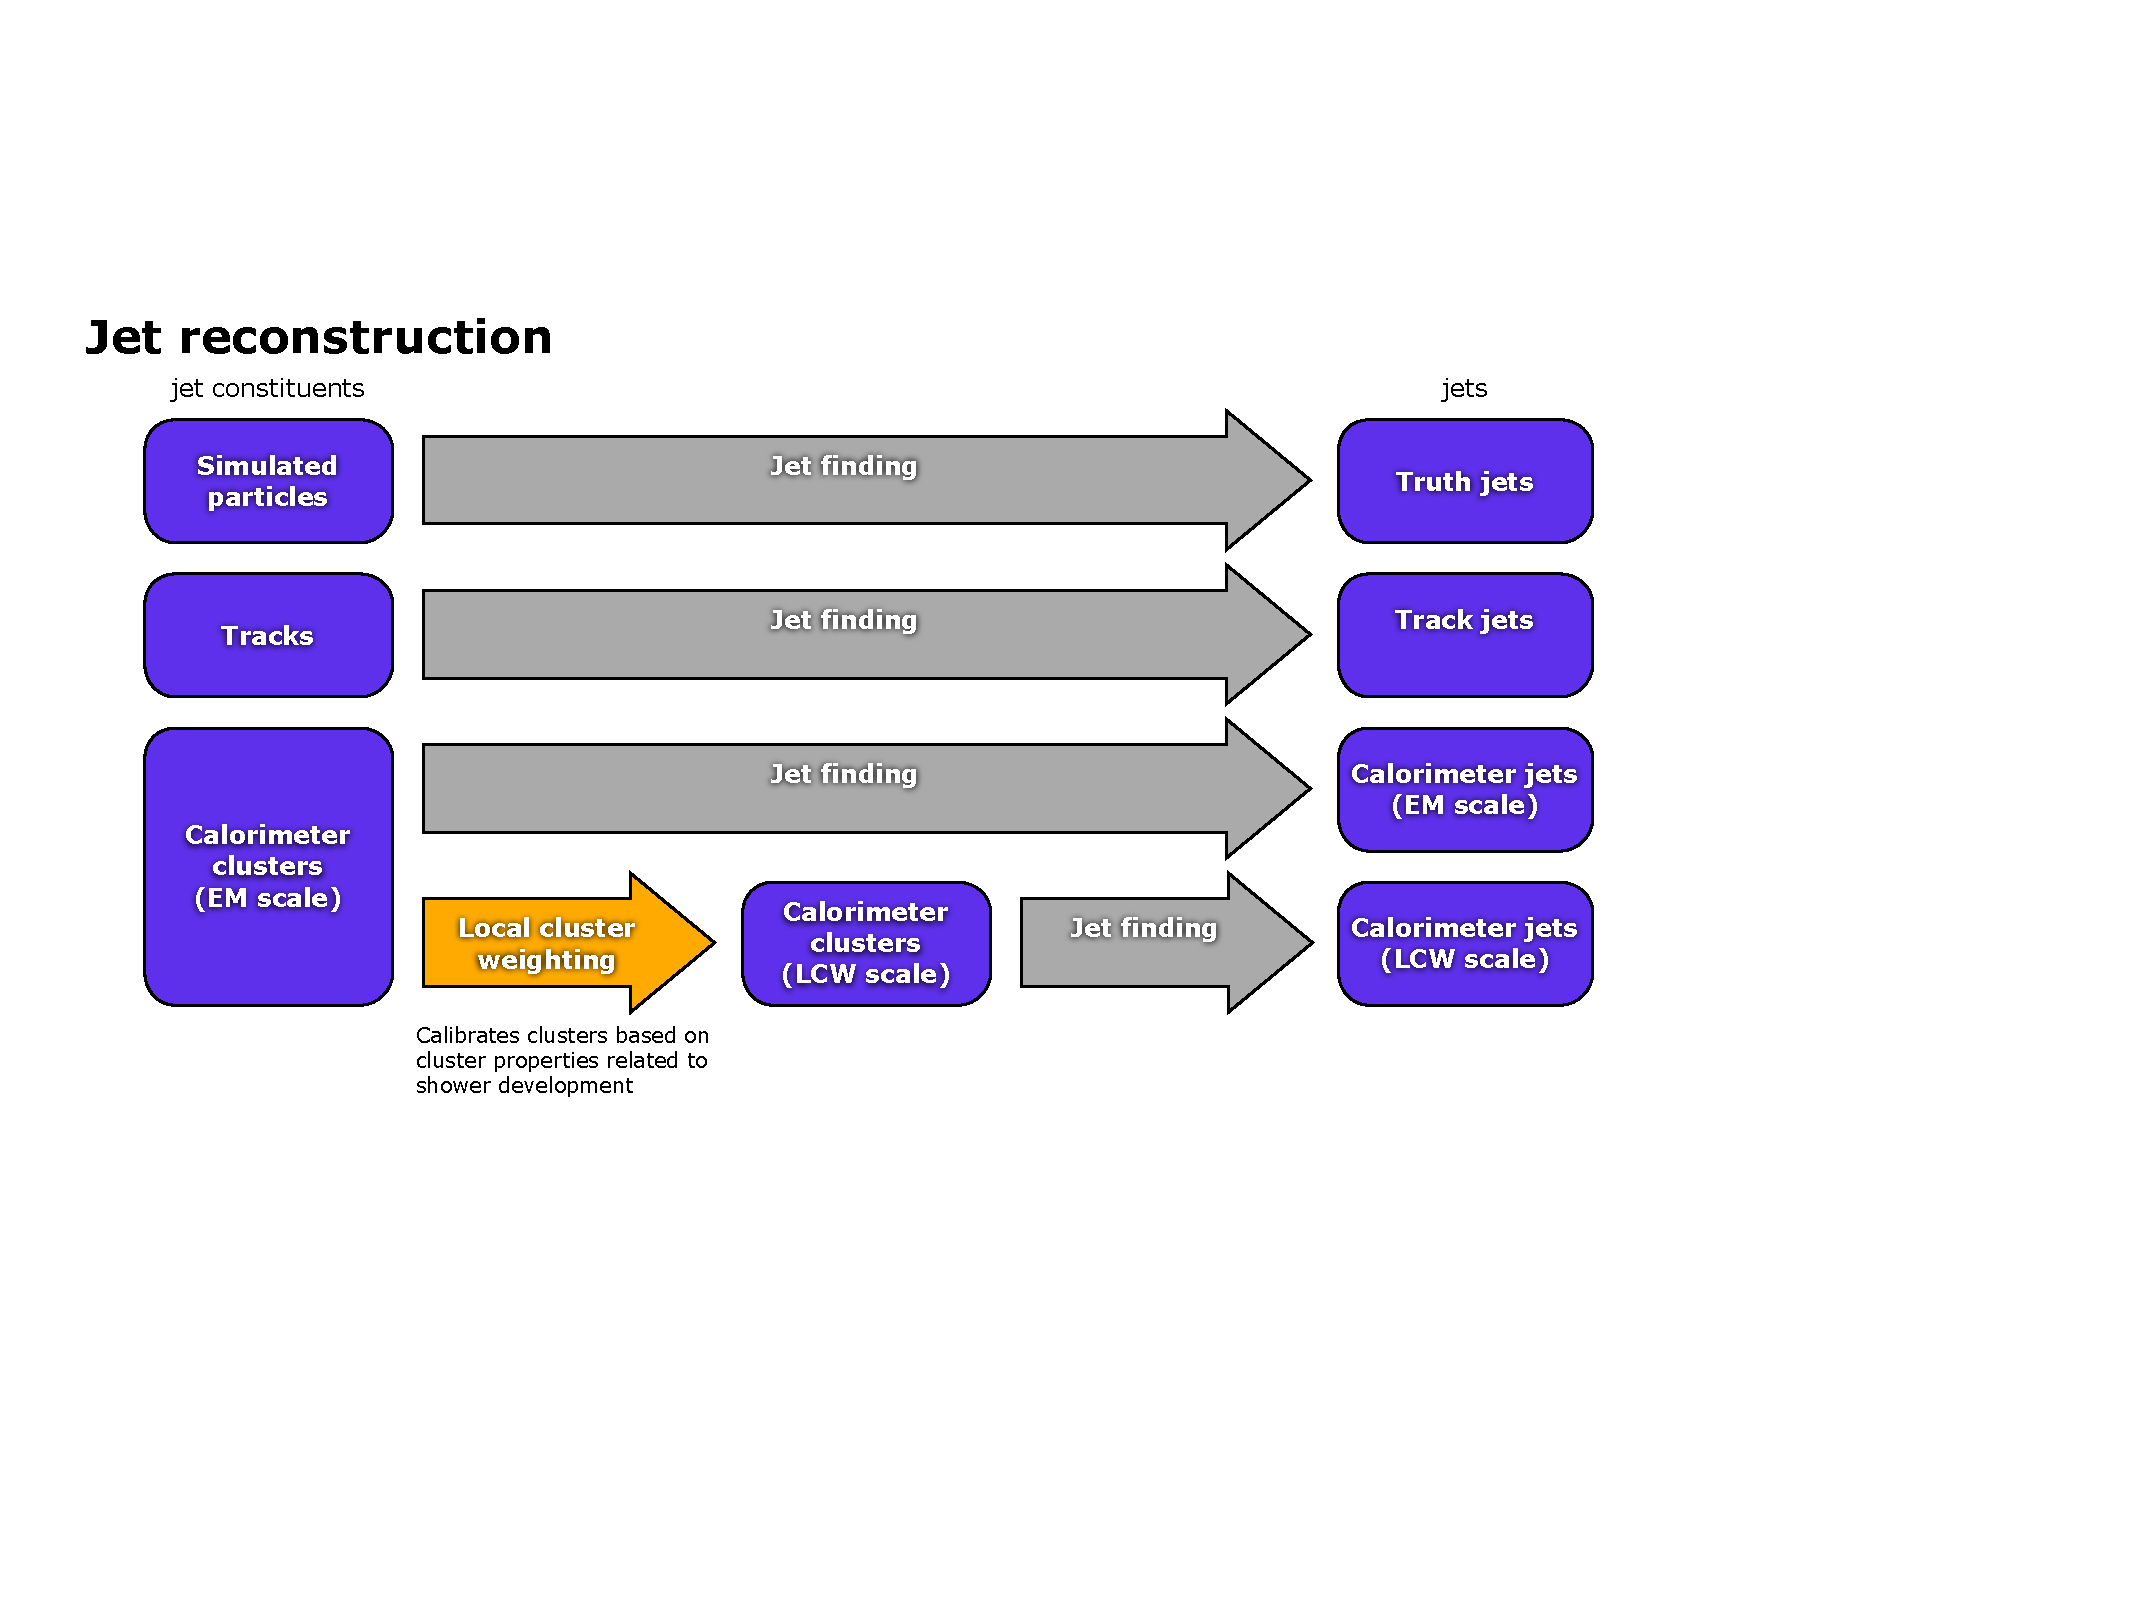
\includegraphics[width=0.7\textwidth]{making-jets.pdf}
\label{fig:jet-reconstruction:making-jets}
\caption{A diagram showing the various forms of jet inputs, and the different types of jets they are used to make.}
\end{figure}

%%%%%%%%%%%%%%%% 

Jets constructed from the simulated particles from a Monte Carlo generator are called \textit{truth jets}: these are primarily used to study the performance of algorithms without the effect of the detector, and to calibrate and define the resolution of other classes of jets. 

Jets can also be constructed from tracks, the outputs of pattern recognition algorithms performed on the hits in the Inner Detector, which correspond to the trajectories of charged particles. These \textit{track jets} are mostly used for validation: they provide a completely independent measurement of a jet from the calorimeter, and while they miss the neutral third of particles, the increased angular precision of tracking can result in complementary information to the calorimeter measurement. \editnote{Cite Seth's thesis, substructure paper?} 

Finally, and most importantly, jets can be formed from energy deposits left in the calorimeter, and these are called \textit{calorimeter jets}. Historically, ATLAS went through many different options for reducing the calorimeter information to a more manageable form for input to jet algorithms-- algorithms such as Global Cell Weighting, Noise Suppressed Towers, and simple projective towers were all eventually disfavored compared to the topo-clustering algorithm described in Section~\ref{jet-reconstruction:jet-inputs:topoclustering}. Calorimeter measurements all share several properties: they provide a measurement of the total energy of the parton shower, produced in both neutral and charged particles. This measurement of the jet (after relevant calibrations are applied) is at approximately the same scale as the quark which initiated it: for example, the invariant mass of the leading non-$b$-tagged jets in semi-leptonic $t\bar{t}$ peaks at the value of the mass of the $W$-boson, $m_{W} = 80$~GeV. Calorimeter jets can thus be used as 4-vectors in the same way that other detector objects-- electrons, photons, etc.-- are used (though of course there is more information in the structure of these jets, which analyses in this thesis do exploit).  \editnote{so many citations needed}

One alternative to separate tracking and calorimeter reconstructions of jets is to use a ``particle flow'' algorithm to combine the measurements from the separate detectors into coherent particle candidates which an be used as inputs to jet algorithms. Such algorithms exploit the fact that charged particles are much more accurately measured (up to some crossing point determined by the strength of the magnetic field) by tracking systems rather than calorimeter systems. Typically, tracks are extrapolated to the calorimeter and matched to energy deposits there; these matched deposits are then subtracted from the calorimeter, as the energy is already accounted for by the tracker. Unmatched energy deposits are assumed to have been created by photons or neutral hadrons, and remain in the list of inputs. Thus, the best features of tracker measurements (accurate energy resolution, and very good angular precision) and calorimeter measurements (capability of measuring neutral particles, good energy resolution at high energies) are combined. The CMS detector is particularly well suited to such reconstruction: the calorimeters are inside the 3.8 T magnetic field (nearly two times stronger than ATLAS), so energy deposits are more widely separated and track-to-calorimeter matching is less ambiguous. Since two thirds of the particles in the jet are reconstructed with tracks instead of calorimeter measurements, the reduced performance of the CMS hadronic calorimeters is also less important. However, as ATLAS has a weaker (and smaller, spatially) magnetic field, and compartively stronger hadronic calorimeters, the improvement from this approached is much diminished and ATLAS has thus far not used the particle flow algorithm for analyses. \editnote{cite cite cite}

The following subsections describe some details of the topoclustering and tracking algorithms which form the inputs to the jet algorithms in ATLAS. The design decisions in these algorithms-- and the strong performance they achieve in the face of difficult operating conditions-- are critical for the final results of hadronic analyses on ATLAS.

\subsection{Topoclustering}
\label{jet-reconstruction:jet-inputs:topoclustering}

\subsection{Tracking}

Discussion of bending, out of cone

\subsubsection{Ghost Association}

Alternative to independent track jets

\subsection{Cluster Calibration}

\section{Jet Calibration}

Once a jet has been clustered, from either EM-scale or LC-scale constituents, it is not yet ready for use by analyses. The non-compensating nature of the ATLAS calorimeters guarantees that the energy measured by the detectors is not the full energy of the particles which passed through them. Jets on ATLAS therefore go through several stages of additional corrections and calibrations, as outlined in Figure~\ref{fig:jet-reconstruction:making-jets}. Each level of the corrections and calibrations is referred to as a \textit{scale}. The steps involved are:

\begin{enumerate}
	\item Jet clustering, producing jets at the \textit{constituent scale} (or EM/LC)
	\item Jet areas pileup correction, and a residual NPV and $\mu$ dependent offset, producing jets at the \textit{pileup corrected scale}
	\item A jet origin correction, correcting the $\eta$ of a jet for the true location of the primary vertex, creating jets at the \textit{origin corrected scale}
	\item A Monte Carlo based \textit{Jet Energy Scale} (JES) calibration, producing jets at the \textit{particle scale}
	\item A Global Sequential Calibration to reduce flavor and hadronization sensitivity
	\item In-situ data-driven calibrations, producing jets at the \textit{fully calibrated scale}
\end{enumerate}

All of these steps are applied in ATLAS to $R=0.4$ and $R=0.6$ jets, using both EM and LC-scale inputs. While the LC calibration of the clusters is able to correct for non-compensation to some extent (by noting the difference between hadronic and electromagnetic interactions in the calorimeter, and the corresponding different energies they deposit), even LC-scale jets require significant further calibrations to correspond to truth jets. \LargeR jets, as used by the analyses in this thesis, undergo only the MC JES calibration, for reasons discussed below. The following sections describe each of these steps in detail.

%%%%%%%%%%%%%%%%

\begin{figure}
\centering
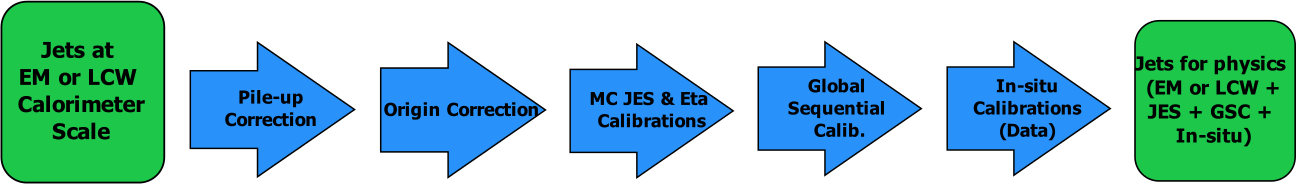
\includegraphics[width=0.6\textwidth]{JES_calib_chain.png}
\label{fig:jet-reconstruction:making-jets}
\caption{A diagram displaying the multiple steps which are used to transform a jet at the constituent scale to a fully-calibrated physics object for use in analysis.}
\end{figure}

%%%%%%%%%%%%%%%% 

\subsection{Pileup Corrections}

The first stage of jet calibration is to correct for pileup. As the calorimeter has a poor pointing resolution\footnote{Except with the notable exception of the ECal presampler, though this information is still limited and not yet used for pileup identification.}, it is not possible to determine which primary vertex (the hard-scatter, or pileup) an energy deposit originated from. This means that as a calorimeter jet is clustered, it contains energy from both the interaction of interest and the additional less-interesting interactions which occurred during the same bunch crossing. Even if a particle-flow algorithm is used to replace charged hadrons with their tracker measurements, thereby allowing a charged-hadron subtraction using the vertex identification of the tracks, neutral pileup particles cannot be subtracted and will add energy to the jet. \editnote{cite cite}

Jet pileup corrections are a broad topic of active research in both the theoretical and experimental community. \editnote{cite cite} The approach currently used by ATLAS is referred to as the \textit{jet areas} technique~\cite{jetareas}. The basic approach is to measure, event-by-event, the \textit{energy density} $\rho$ in the calorimeter. Though the underlying event contributes, at moderate and higher ($\mu > 10$, approximately) numbers of interactions, the contribution due to pileup to the energy density is dominant. Once the event energy density is measured, and the \textit{jet area} is measured, it is a simple matter to multiply the two and subtract off the pileup contribution to a jet.

The energy density can be measured in many ways. One approach, currently favored in the theory community, is simply to use sliding grid-shaped windows to scan the calorimeter, measuring the total energy deposit in each window, and then taking the median. The median is the best estimate of the ambient energy: measures such as the mean can be biased by the actual hard-scatter jets in the event. The approach used by ATLAS is similar, and follows an older prescription from the authors: the event is clustered into \kt $R=0.4$ jets, and each of their areas is calculated using the \textit{voronoi} technique (described below). The energy/area is calculated for each jet, and the median is used as the energy density (again in order to exclude outliers from real jets).

One detail of the topo-clustering algorithm creates an interesting effect when calculating the energy density. At approximately $\eta = 2.5$, the detector transitions from the barrel to the end-caps, which have a much higher expected noise due to pileup, as discussed in Section~\ref{jet-reconstruction:jet-inputs:topoclustering}. This, along with the reduced granularity in the forward regions, means that the energy density outside of jets decreases substantially: jets themselves are often still energetic enough to go over the noise thresholds required for topocluster formation, but pileup is often not. Thus, when calculating $\rho$, it is important to exclude the forward region of the detector, as the ambient energy outside of jets has greatly different characteristics than in the central region.

There are also several ways of calculating the area of jets, the simplest of which is the voronoi technique previously mentioned. A voronoi algorithm tiles a space (the calorimeter in $y-\phi$ space, in this case) such that each tile contains only one element (i.e., only one topocluster), and each tile contains all the points that are closest to that tile's element compared to any other~\cite{catchmentarea}. The voronoi area has the advantage of being fast to calculate, and gives (on average) the same value as more expensive calculations. The largest issue is that the algorithm does not take into account the energy of each element, which does not reflect the fact that the $k_T$ distance metrics generally do use energy.

A more sophisticated treatment of the area of a jet asks the question ``if a particle with very, very low energy were is at some position $\eta,\phi$, which jet (if any) would it join?'' This concept is at the heart of the \textit{catchment area} of a jet~\cite{catchmentarea}. To measure this area, special \textit{ghost particles} representing locations in the calorimeter participate in the jet clustering. The ghost particles have negligible energy (typically set to some $\epsilon$ value above 0), and so the IRC safety of the $k_T$ algorithms guarantee that the ghosts do not affect the clustering of the real jets. Once the mixture of ghost particles and real particles is clustered, one can examine which jet the ghost particle joined. When enough ghosts are used, this can be used to define the area of a jet (up to some level of coarseness). If the ghosts representing all the different calorimeter points are all simultaneously clustered with the real particles, this is referred to as the \textit{active area}; if on the other hand each point is added to the particles individually, and a separate clustering run each time, this is referred to as the \textit{passive area}. Both techniques are much slower than the Voronoi area calculation, and the passive calculation is again much slower than the active. The best compromise in terms of performance and usefulness of results seems to be the active area, and this is the definition used by ATLAS. The catchment area solves the issue observed with the Voronoi area: jet boundaries are determined by the algorithm's properties, and not just the closest point of a cluster. \Antikt jets, for example, form circles in $y-\phi$, and overlapping jets favor the higher $p_T$ jet: the $p_T$ weighting of the algorithm means that if a particle could join one of two jets, it will join the one with more energy. Figure~\ref{fig:jet-reconstruction:jet-active-areas} shows an event display with the areas of many \antikt $R=1.0$ jets and their \kt $R=0.3$ subjets: the circular nature of the \antikt algorith, and the more chaotic nature of \kt, are both visible.

%%%%%%%%%%%%%%%%

\begin{figure}
\centering
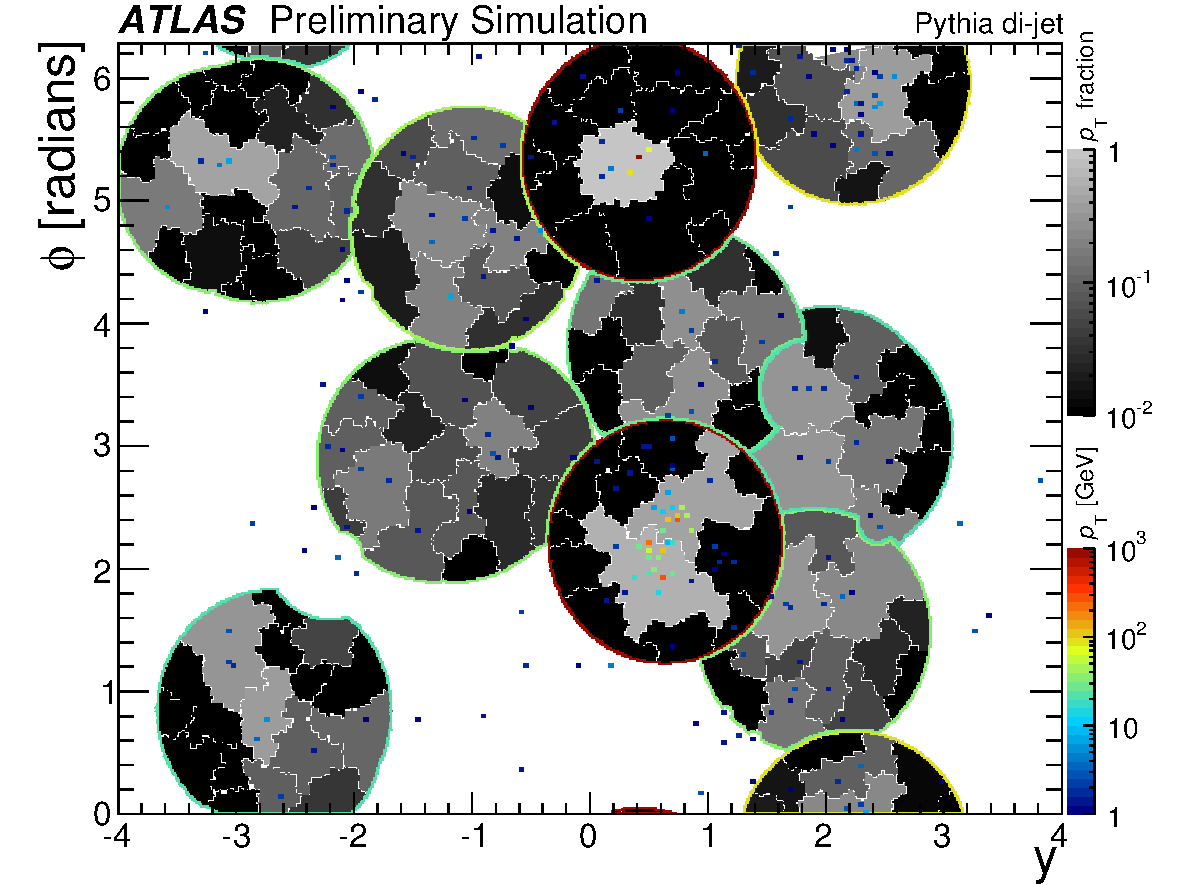
\includegraphics[width=0.6\textwidth]{jet-areas-example.pdf}
\label{fig:jet-reconstruction:jet-active-areas}
\caption{An event display showing a Pythia QCD simulation event with \antikt $R=1.0$ trimmed jets, with subjets formed by the \kt algorithm with $\Rsub = 0.3$.}
\end{figure}

%%%%%%%%%%%%%%%% 

Once the jet area and the energy density are known, the jet can be corrected. There are two approaches to this-- the simpler one is referred to as the scalar correction, and is applied with:
%
\begin{equation}
p_T^{\mathrm{corrected}} = p_T - \rho A
\end{equation}
%
where $A$ is the scalar area of the jet. It is also common to define the 4-vector $A_\mu$ by treating each ghost as a 4-vector and taking the sum of all of these; this allows for the 4-vector correction:
%
\begin{equation}
p_\mu^{\mathrm{corrected}} = p_\mu - \rho A_\mu
\end{equation}
%
Often this is preferable, as not just the $p_T$ but the mass of the jet is thus corrected for pileup. However, in some situations it is possible for the jet mass to be over-corrected, resulting in a negative $m^2$ and therefore imaginary mass. For this reason, ATLAS used only the scalar correction in Run~1. After the pileup correction, a jet is referred to as being at the ``pileup corrected scale'' and is ready for further calibration. Figure~\ref{fig:jet-reconstruction:jet-pu-vs-mu} shows the improvement in the RMS of the jet offset-- a measurement of the resolution induced by pileup-- as a function of $\mu$. The corrected distribution in blue shows a substantial improvement over the original distribution in black, and an average NPV based correction in red.

%%%%%%%%%%%%%%%%

\begin{figure}
\centering
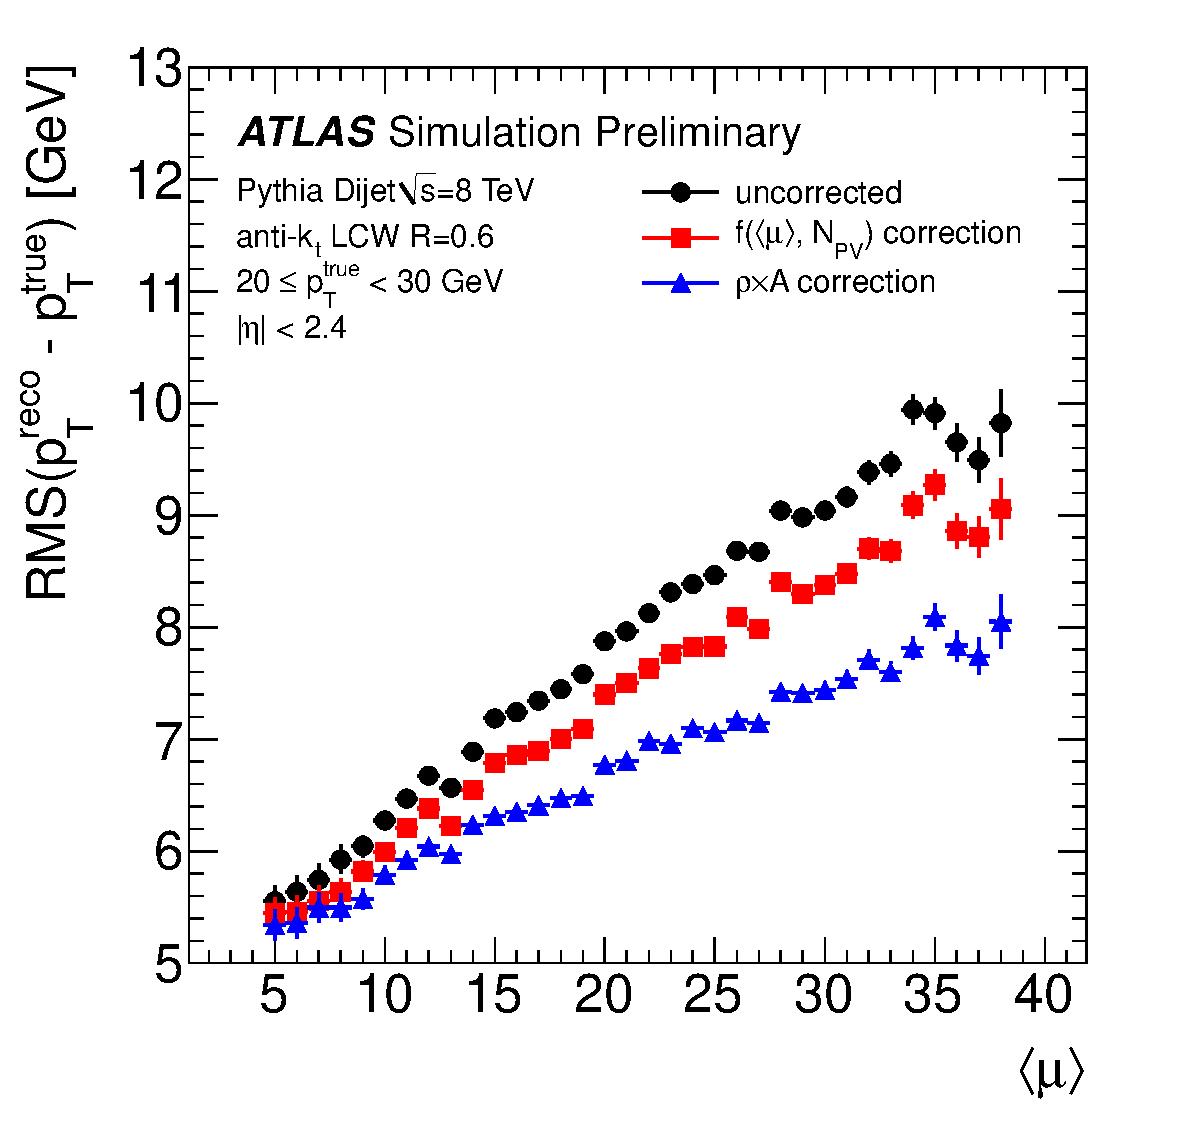
\includegraphics[width=0.6\textwidth]{pu_vs_mu.pdf}
\label{fig:jet-reconstruction:jet-pu-vs-mu}
\caption{The improvement of the width of the jet offset (a measurement of the jet resolution in simulation) from the application of the jet areas pileup correction in blue, compared to an NPV based correction in red, and no correction in black.}
\end{figure}

%%%%%%%%%%%%%%%% 

One important aspect to note is that these corrections are done on jet 4-vectors as a whole, and not on constituents-- this means that jet moments, such as substructure observables, are not corrected. There are several extensions of the areas technique which aim to correct shapes, and some additional ideas which correct jet inputs before clustering, and therefore automatically correct shapes. While ATLAS explored some of these options in Run 1, the susceptibility of most variables to pileup was found to be rather small, putting off the need for dedicated corrections to Run 2. \editnote{cite, cite}


% plots plots? summarizing this?

%origin correction?

\subsection{Jet Origin Correction}

...

\subsection{MC Jet Energy Scale}
\label{jet-reconstruction:jet-calibration-mc-jet-energy-scale}

The MC Jet Energy Scale is the next step of the jet calibration chain. The sampling and non-compensating nature of the ATLAS calorimeters means that the measured energy is only some fraction of the energy of the actual particles passing through the detector. Futhermore, as the detector technology changes as a function of $\eta$, topoclusters in different parts of the detector may be better or worse measured, leading to biases in the jet direction. The JES is a correction which restores (on average) both this full energy, and correct direction, of a measured jet~\cite{JES2010}. The calibration is a multiplicative correction on energy, and an additive correction on $\eta$, binned in both the reconstructed jet energy and $\eta$.

Jets, composed of either EM or LC-scale clusters, are calibrated to the particle scale\footnote{From now on, reconstructed jets will refer to jets of both EM and LC consituents.} in Pythia 8 dijet events. This requires that the reconstructed jets are matched to truth jets. The requirement for matching is such that the $\Delta R$ between the reconstructed and truth jet is $<0.75\times R$. Furthermore, the matched jets (both truth and reconstructed) are also required to be isolated, such that no other jet of its type exists within $\Delta R < 2.5\times R$. All well matched jets within the sample are used. The dijet sample is used because it produces a well-understood spectrum of jets at many energy scales. The energy response is defined as:
%
\begin{equation}
\mathcal{R}^{\mathrm{jet}} = E^{\mathrm{jet}}_{\mathrm{reco}} /  E^{\mathrm{jet}}_{\mathrm{truth}} 
\end{equation}
%
and is measured in fine bins of $\eta_{\mathrm{detector}}$\footnote{The detector $\eta$ is used as it corresponds better to the location of the jet in the calorimeter.} and $E^{\mathrm{jet}}_{\mathrm{truth}}$. Each bin produces a Gaussian distribution, which is fit and the mean value is extracted. Each $E^{\mathrm{jet}}_{\mathrm{truth}}$ point in an $\eta$ bin then is then transformed into the corresponding $E^{\mathrm{jet}}_{\mathrm{reco}}$ point by this measured response-- this step is the ``numerical inversion'' which gives the technique its name. An entire $\eta$ bin is then fit by a log-polynomial function, of the form
%
\begin{equation}
\mathcal{F}_\mathrm{calib}\left(E^{\mathrm{jet}}_{\mathrm{reco}}\right) = \sum_{i=0}^N a_i \ln \left( E^{\mathrm{jet}}_{\mathrm{reco}} \right)^i
\end{equation}
%
where $N$, the maximum order of the polynomial, extends from 1 to 6 and is determined by minimizing the $\chi^2/$NDF of each fit. Finally, this function is inverted to get the calibration correction:
%
\begin{equation}
E^{\mathrm{jet}}_{\mathrm{JES}} = \frac{E^{\mathrm{jet}}_{\mathrm{reco}}}{\mathcal{F}_\mathrm{calib}}.
\end{equation}
%
Figure~\ref{fig:jet-reconstruction:e-fit} shows an example of the Gaussian fit used to find the response in each energy and $\eta$ bin; Figure~\ref{fig:jet-reconstruction:ni-e} shows the result of an example fit for the full energy distribution in the same $\eta$ bin. Figure~\ref{fig:jet-reconstruction:calib-function} shows the calibration function for all of the standard jet collections for one bin of $\eta$. Finally, Figure~\ref{fig:jet-reconstruction:total_jes} shows the JES for different energy bins as a function of the detector $\eta$, for both the EM and LC $R=0.4$ collections.

This is a rather complicated procedure, and a relevant question to ask is why the correction cannot be derived by simply measuring the correction factor directly in bins of $E$ and $\eta$, and skipping the numerical inversion steps. The numerical inversion technique, while introducing complexity, is preferred because it removes the dependence of the calibration on the input $p_T$ spectrum. If the correction were binned in $E_{\mathrm{reco}}$, then the truth-jets matched to the reconstructed jet will have both up-fluctuations and down fluctuations due to the calorimeter response, but there are more likely to be down fluctuations, because there are more low $p_T$ jets in the dijet sample than high $p_T$ jets. This introduces a bias due to the $p_T$ shape-- if that shape changes, as it does in a different physics sample, then the calibration would no longer be valid. On the other hand, if we bin in $E_{\mathrm{truth}}$ to start, then the fluctuations up and down will depend only on the calorimeter response-- the physics spectrum has already been accounted for by the $E_{\mathrm{truth}}$ binning.


%%%%%%%%%%%%%%%%

\begin{figure}
\centering
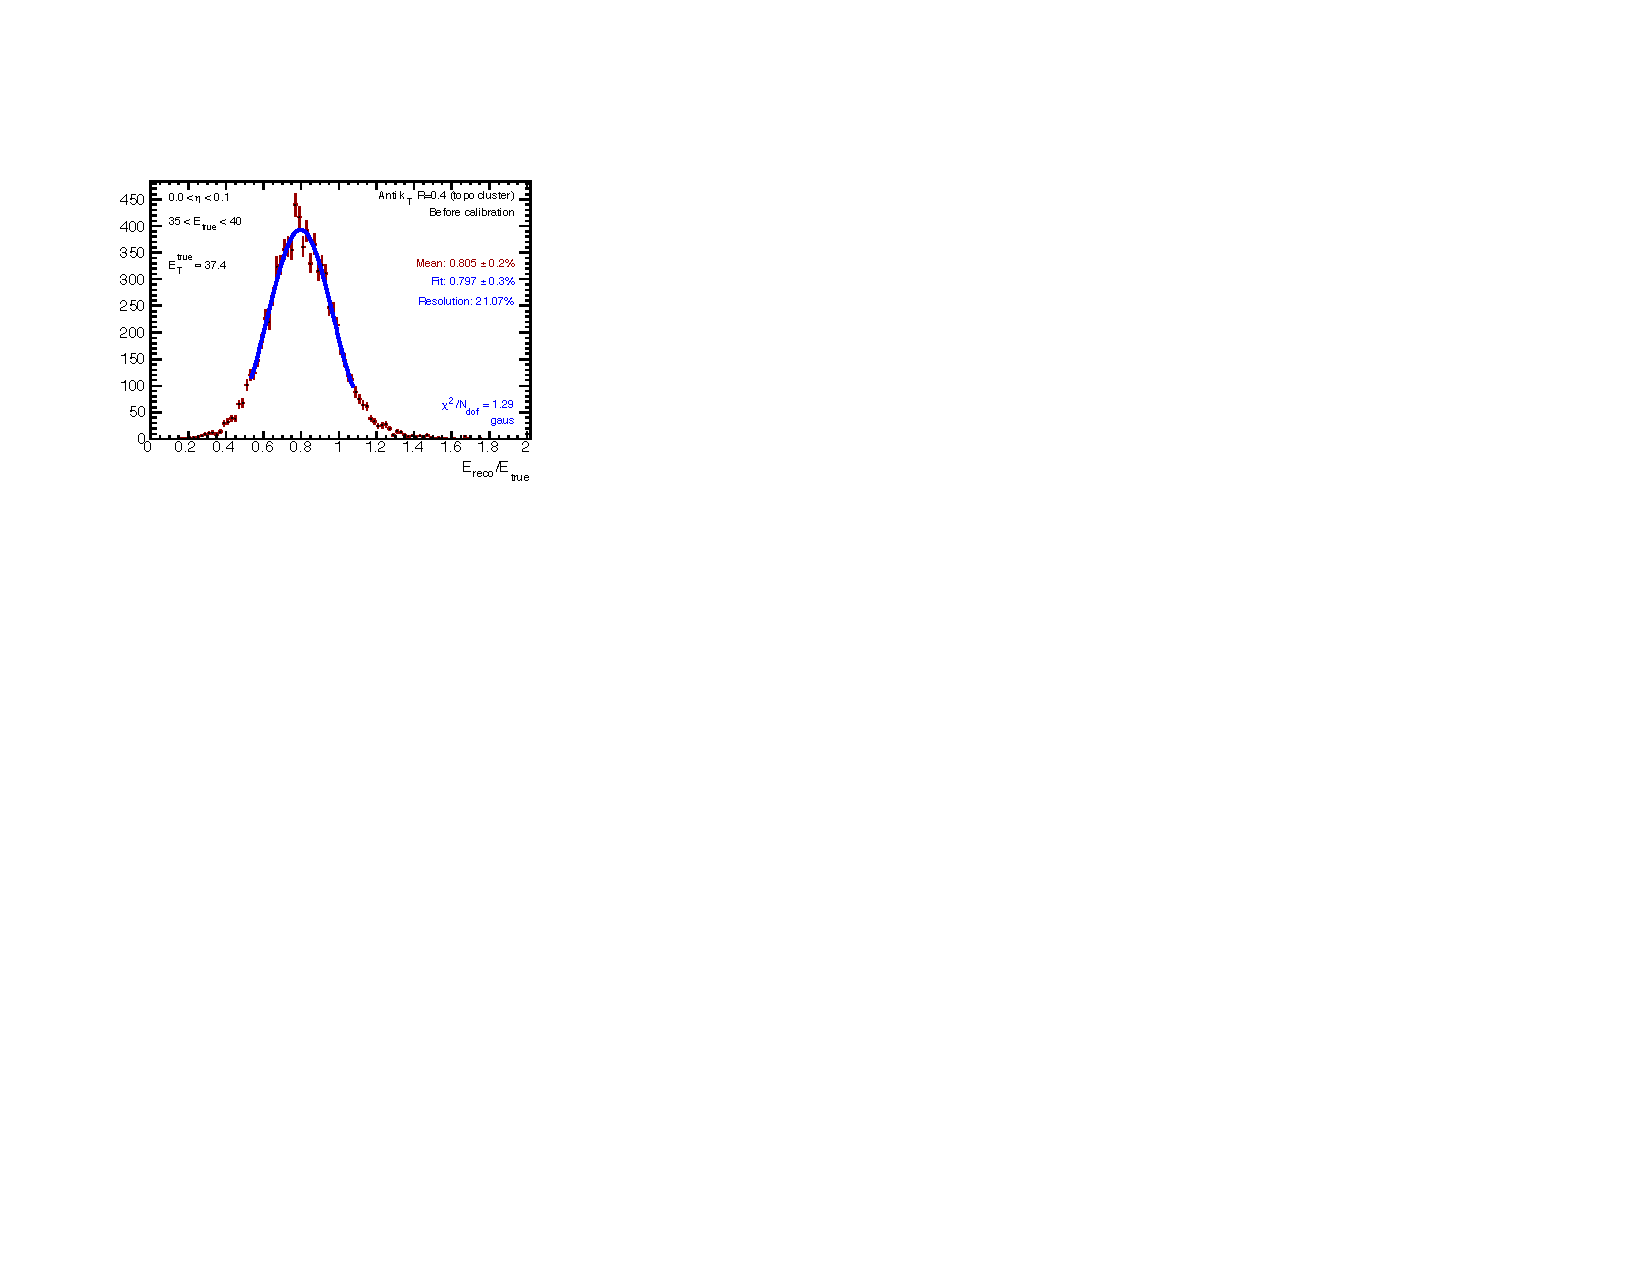
\includegraphics[width=0.6\textwidth]{e_fit.pdf}
\label{fig:jet-reconstruction:e-fit}
\caption{An example of the Gaussian fit used to measure the energy response in a $\eta_\mathrm{detector}$, $E_\mathrm{true}$ bin.}
\end{figure}

%%%%%%%%%%%%%%%% 


%%%%%%%%%%%%%%%%

\begin{figure}
\centering
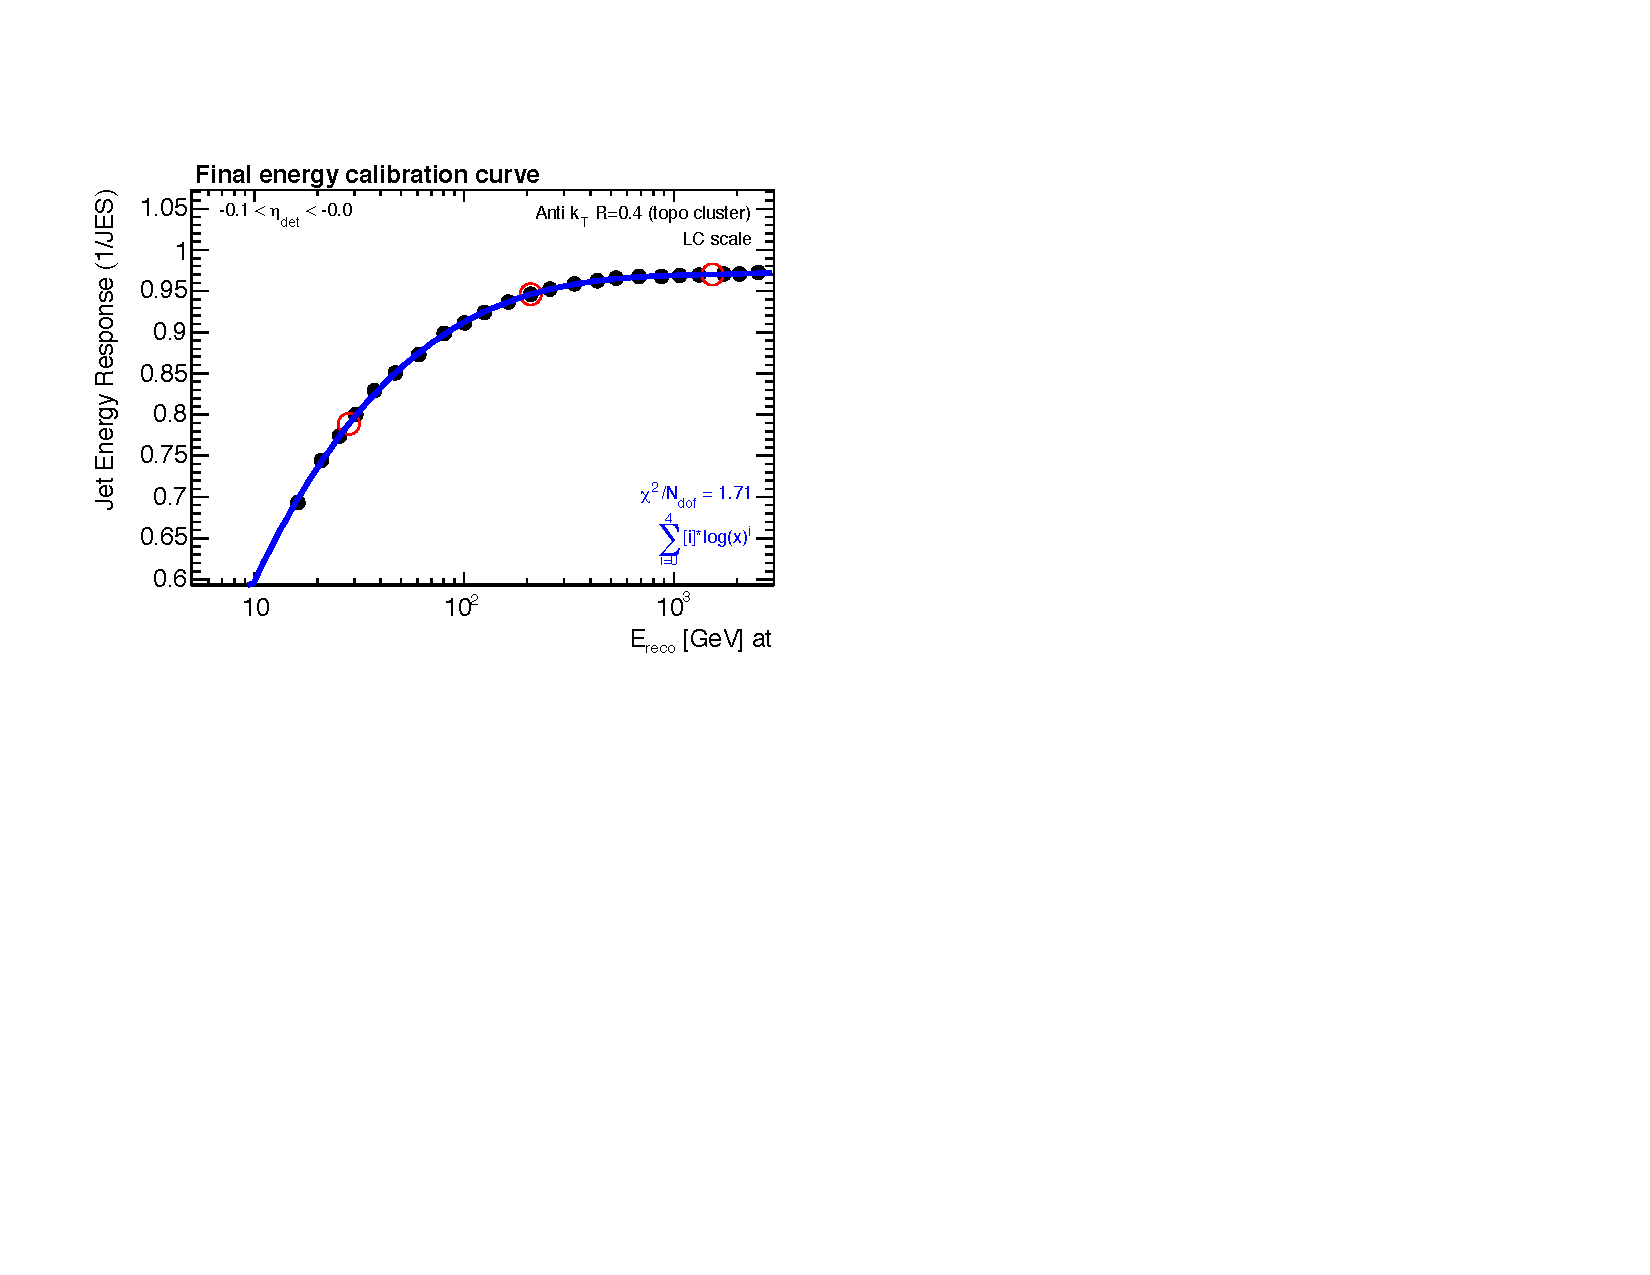
\includegraphics[width=0.6\textwidth]{ni_e.pdf}
\label{fig:jet-reconstruction:ni-e}
\caption{An example of the log-polynomial fit used to measure the jet response as a function of $E_\mathrm{reco}$ in a bin of $E_\mathrm{detector}$. The inverse of this function is the energy calibration applied for each point.}
\end{figure}

%%%%%%%%%%%%%%%% 

%%%%%%%%%%%%%%%%

\begin{figure}
\centering
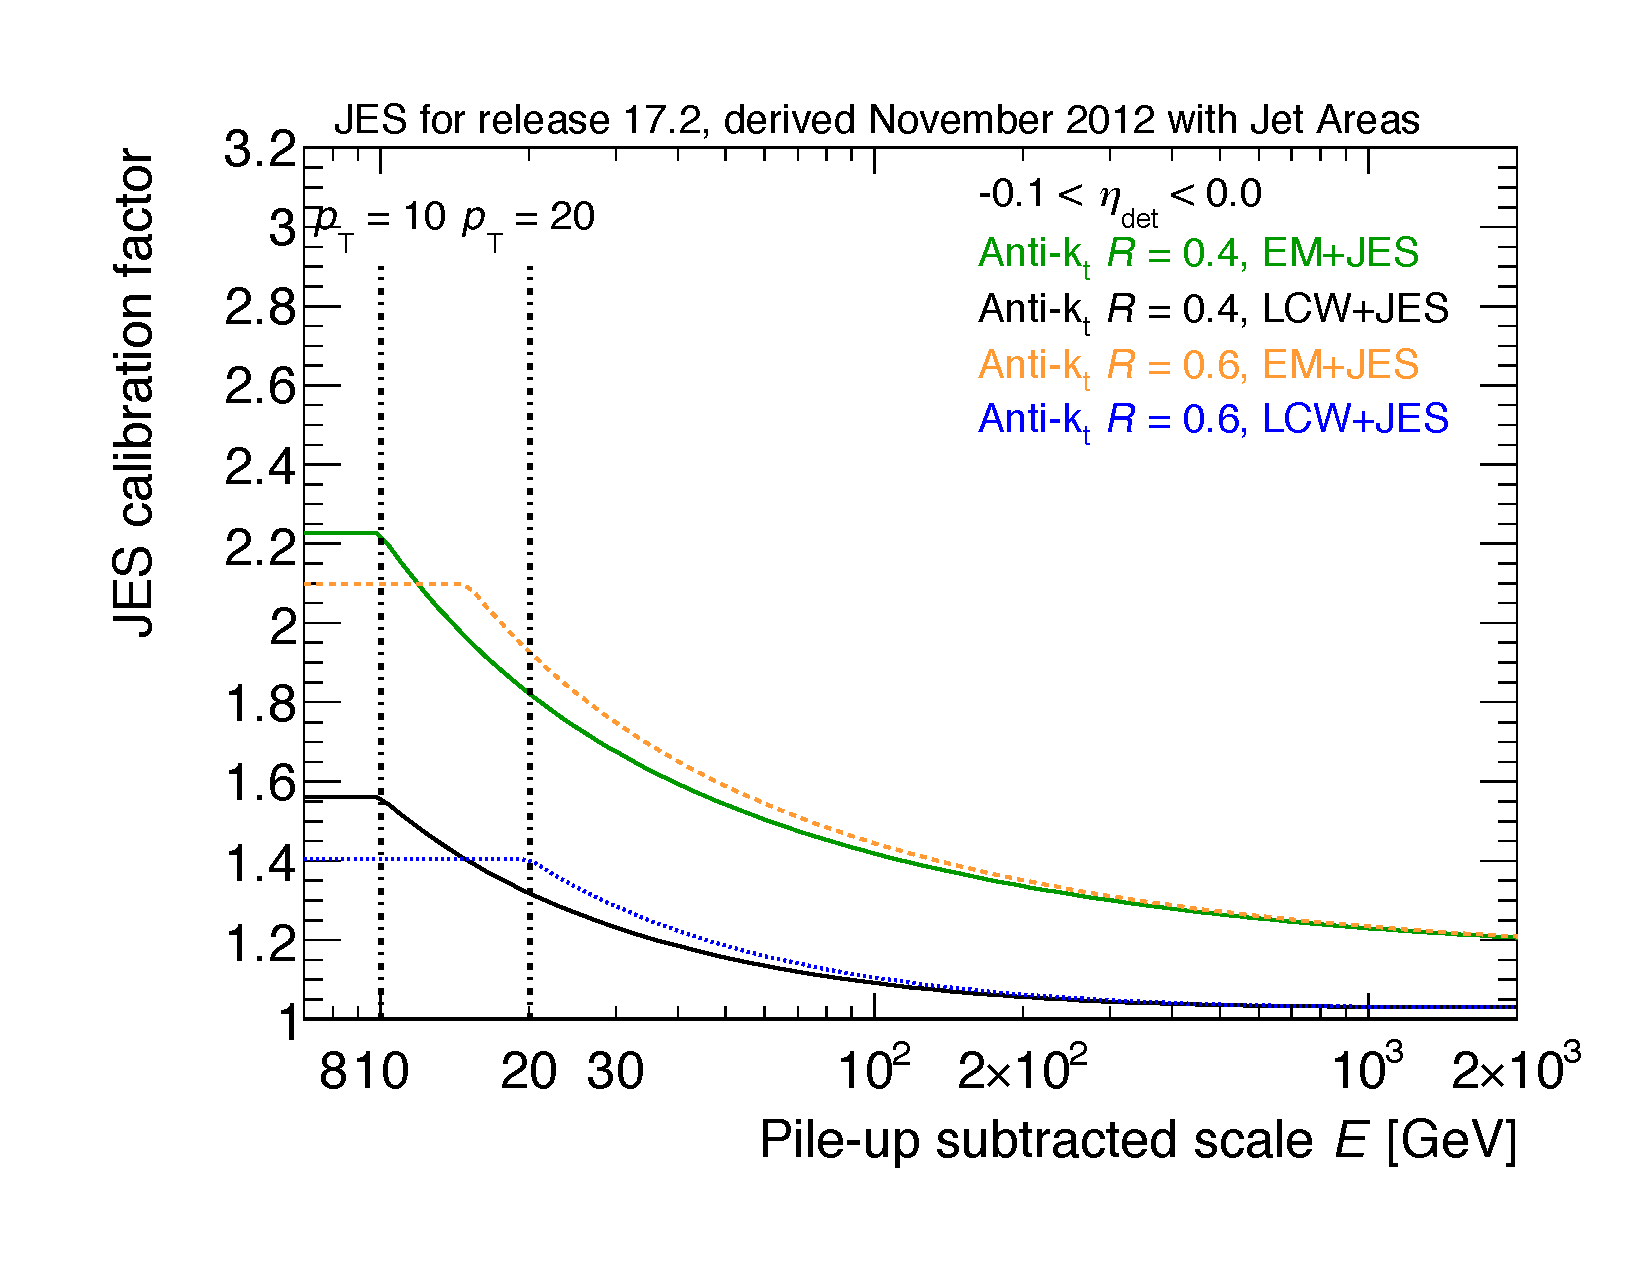
\includegraphics[width=0.6\textwidth]{calib_function.pdf}
\label{fig:jet-reconstruction:calib-function}
\caption{The size of the calibration constants for each of the standard jet collection for one bin of $\eta_\mathrm{detector}$.}
\end{figure}

%%%%%%%%%%%%%%%% 

%%%%%%%%%%%%%%%%

\begin{figure}
\centering
\subfigure[EM]{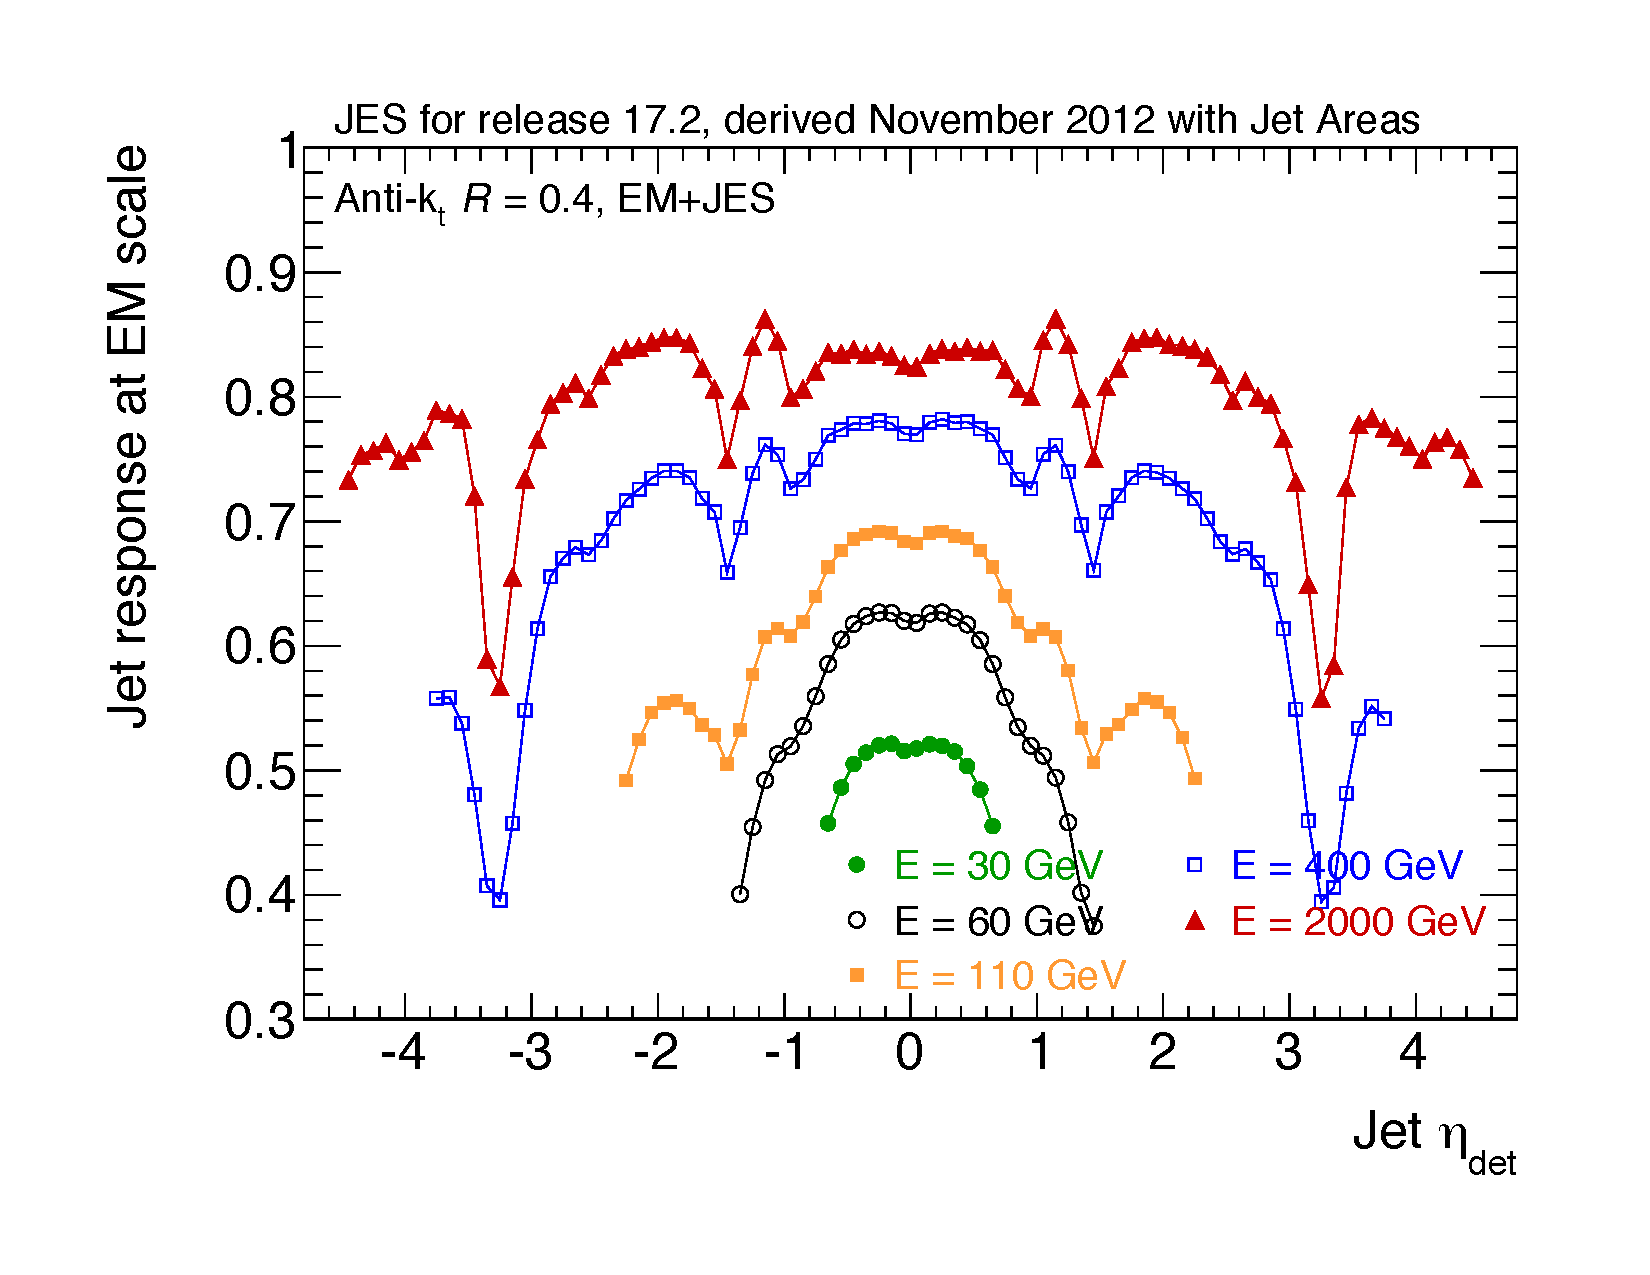
\includegraphics[width=0.45\textwidth]{figures/jet-reconstruction/total_jes_eta_em.pdf}}
\subfigure[LC]{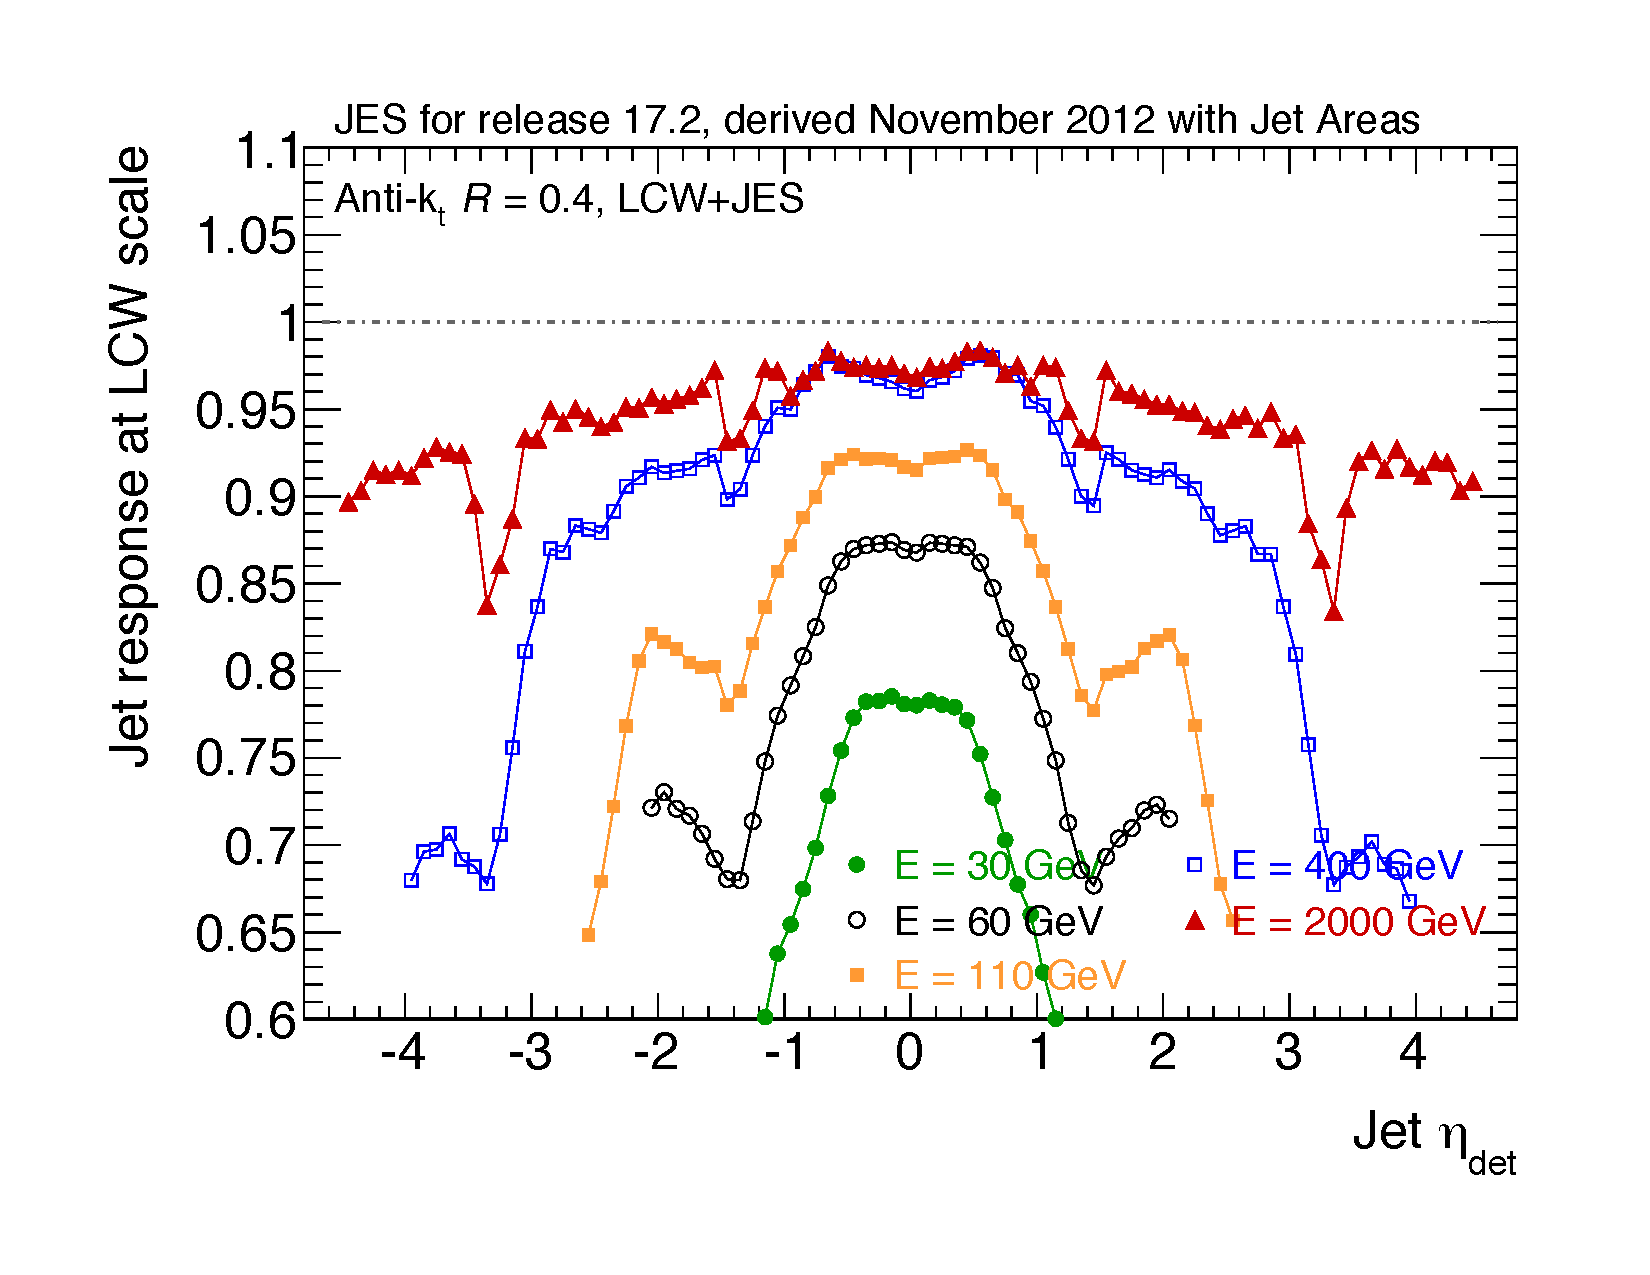
\includegraphics[width=0.45\textwidth]{figures/jet-reconstruction/total_jes_eta_lc.pdf}}
\label{fig:jet-reconstruction:total_jes}
\caption{The size of the calibration constants for each of the standard jet collection for one bin of $\eta_\mathrm{detector}$.}
\end{figure}

%%%%%%%%%%%%%%%% 

The $\eta$ correction mentioned previously is derived as a subsequent correction in much the same way, except that the response is defined additively:
%
\begin{equation}
\mathcal{R}_\eta^\mathrm{jet} = \eta^{\mathrm{jet}}_{\mathrm{reco}} -  \eta^{\mathrm{jet}}_{\mathrm{truth}} 
\end{equation}
%
and the correction is therefore also additive. The size of the correction is not large in the central region, where the uniform detector technology leads to consistently measured clusters, but becomes important especially in the tranisition regions between detectors. Figure~\ref{fig:jet-reconstruction:eta-fit} shows an example of the Gaussian fit used to determine the response; Figure~\ref{fig:jet-reconstruction:ni-eta} shows an example of the calibration function itself in an $\eta$ bin where the correction is non-negligible. Finally, Figure~\ref{fig:jet-reconstruction:total-eta} shows the full size of the correction for different energy bins as a function of $\eta$ for $R=0.6$ EM jets in 2010-- the correction is similar in 2012 conditions.

%%%%%%%%%%%%%%%%

\begin{figure}
\centering
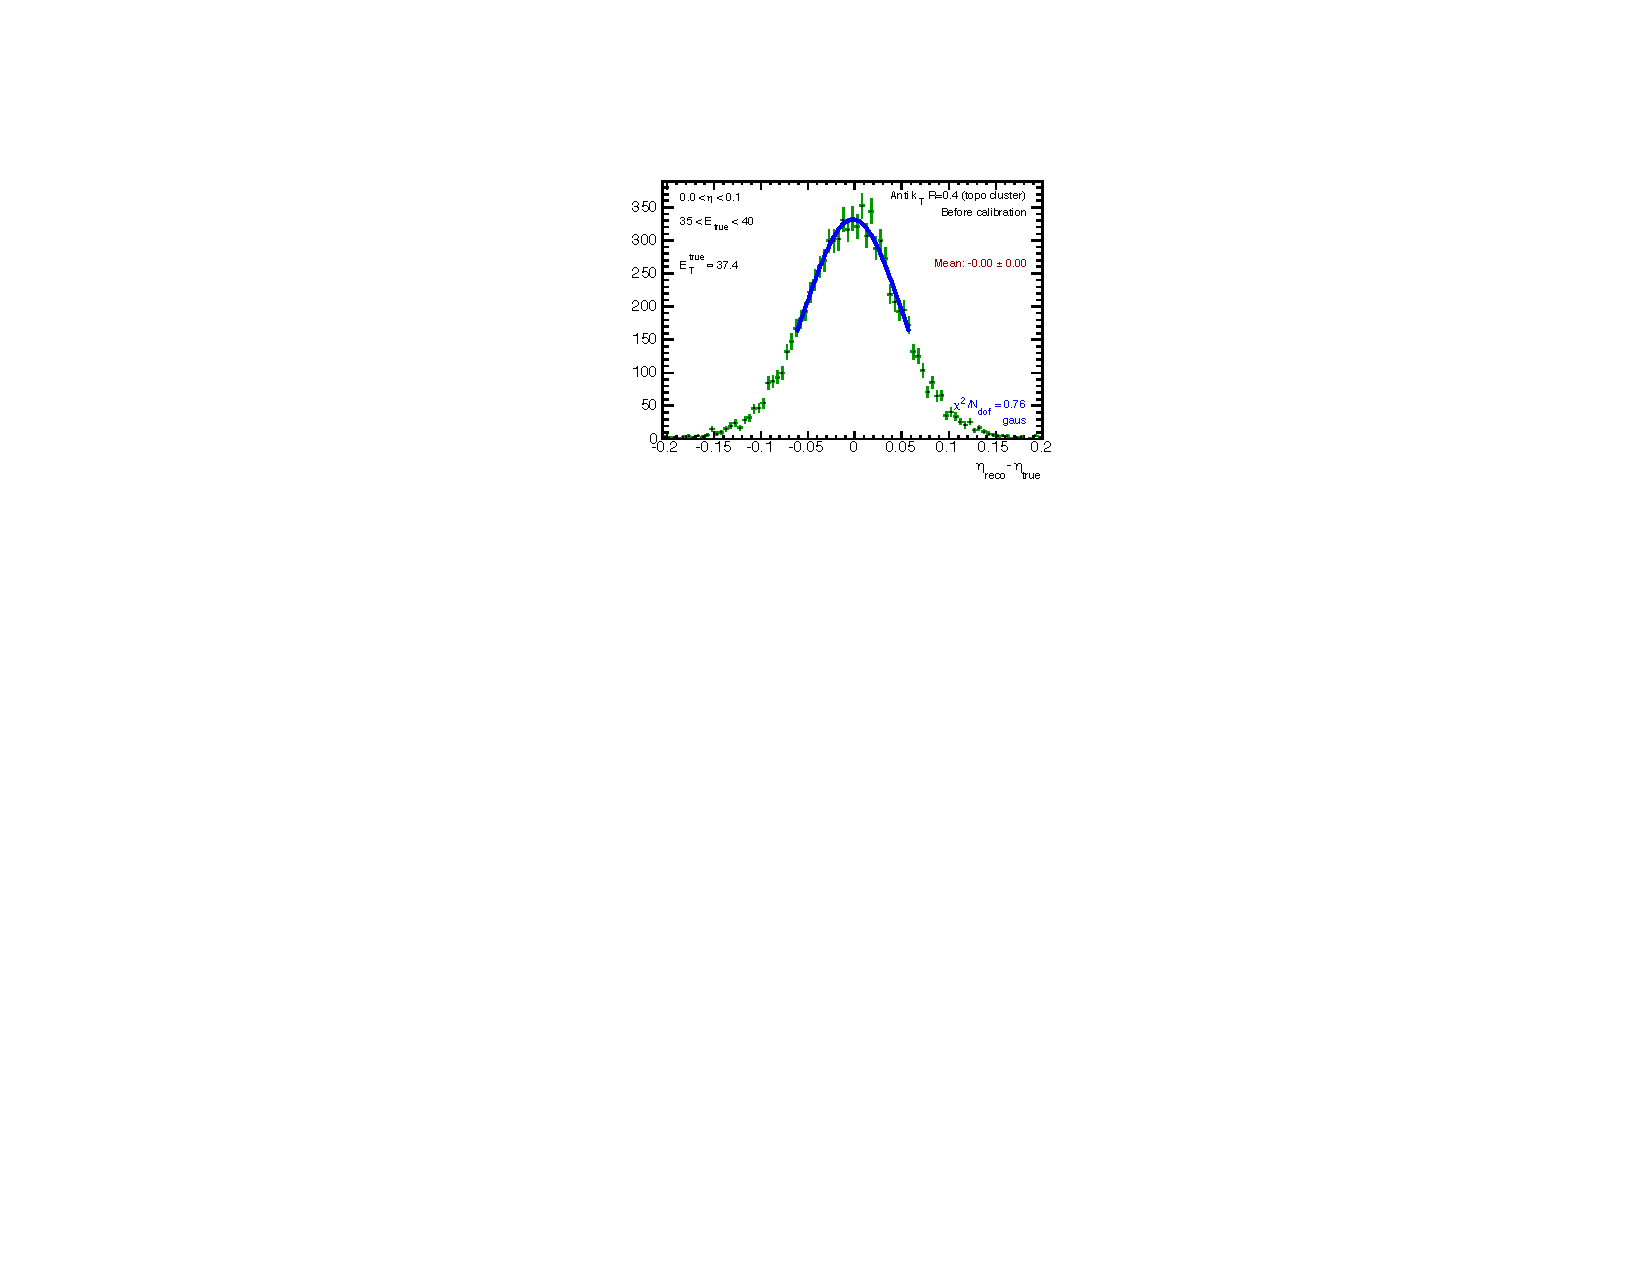
\includegraphics[width=0.6\textwidth]{eta_fit.pdf}
\label{fig:jet-reconstruction:eta-fit}
\caption{An example of the Gaussian fit used to measure the $\eta$ response in a $\eta_\mathrm{detector}$, $E_\mathrm{true}$ bin.}
\end{figure}

%%%%%%%%%%%%%%%%

%%%%%%%%%%%%%%%%

\begin{figure}
\centering
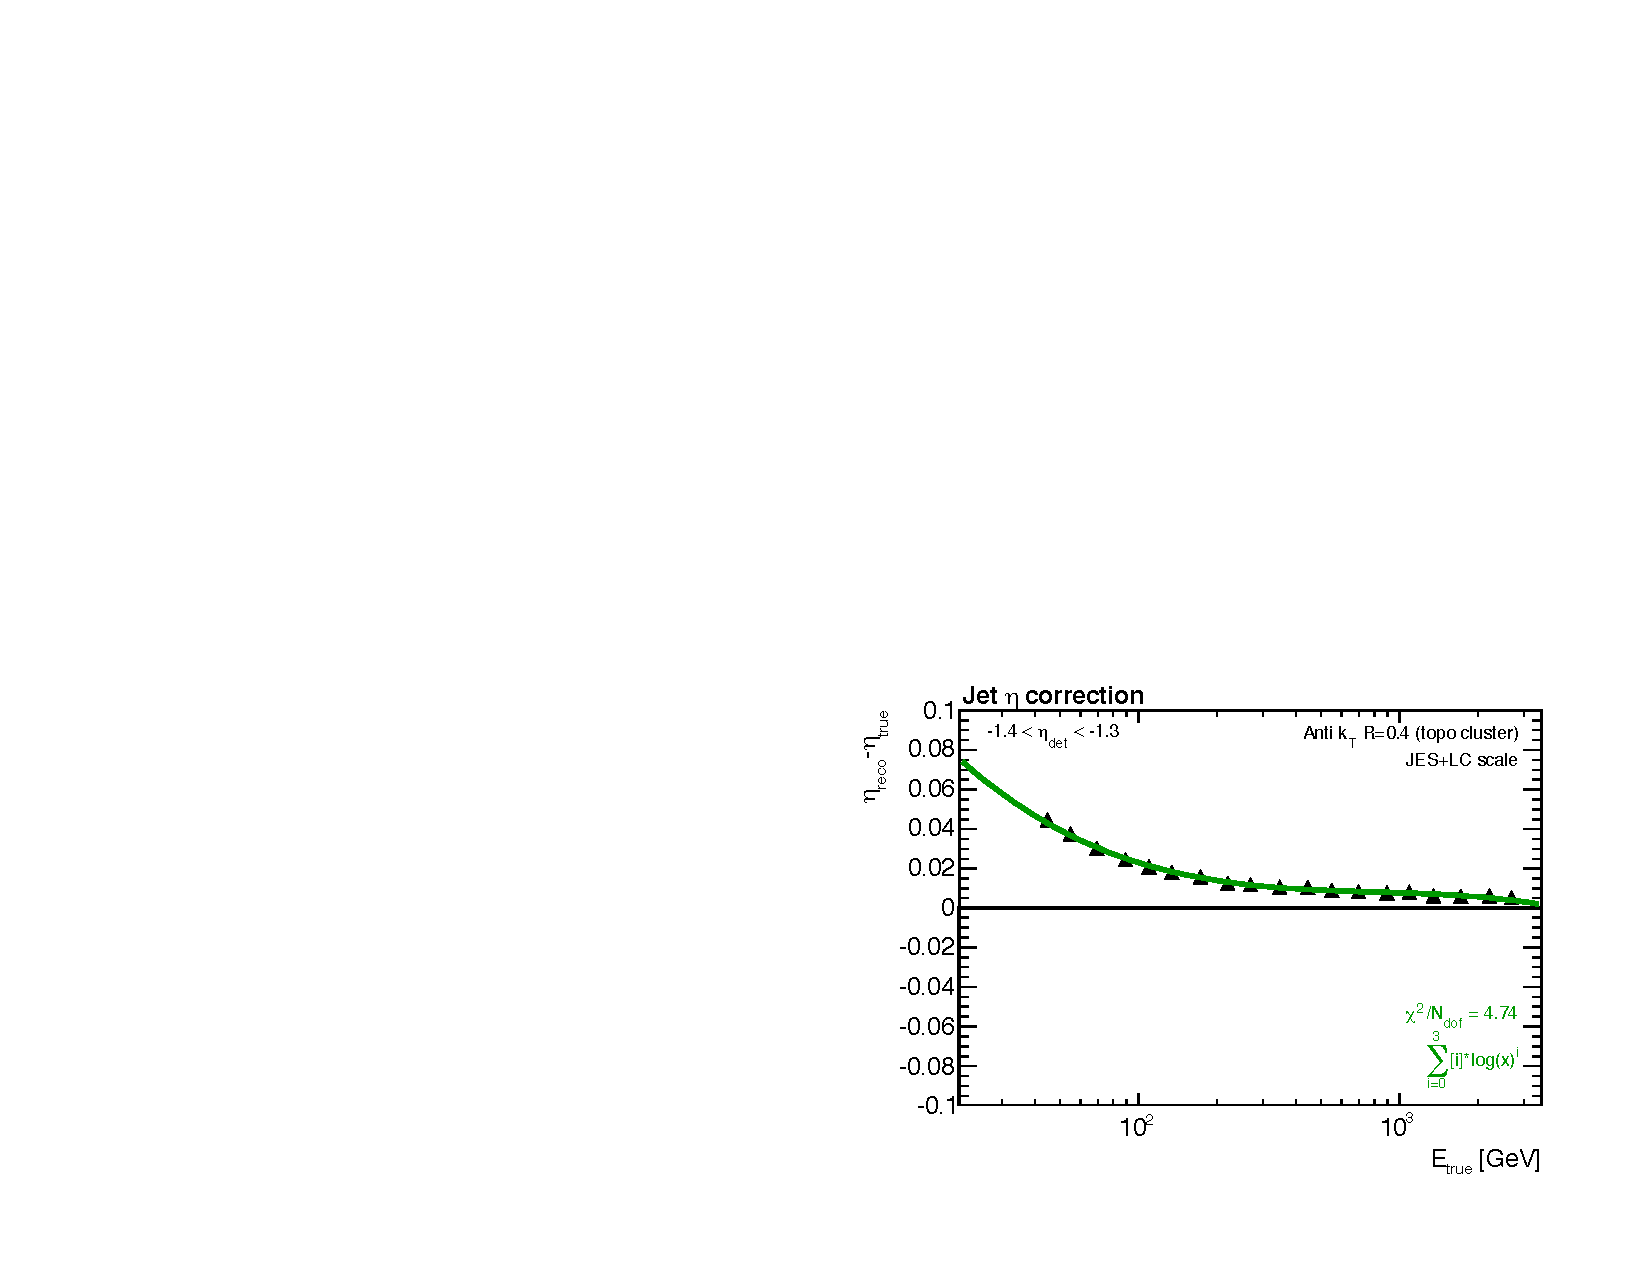
\includegraphics[width=0.6\textwidth]{ni_eta.pdf}
\label{fig:jet-reconstruction:ni-eta}
\caption{An example of the log-polynomial fit used to measure the jet $\eta$-response as a function of $E_\mathrm{true}$ in a bin of $E_\mathrm{detector}$. The jet-$\eta$ correction is the negative of each point.}
\end{figure}

%%%%%%%%%%%%%%%% 

%%%%%%%%%%%%%%%%

\begin{figure}
\centering
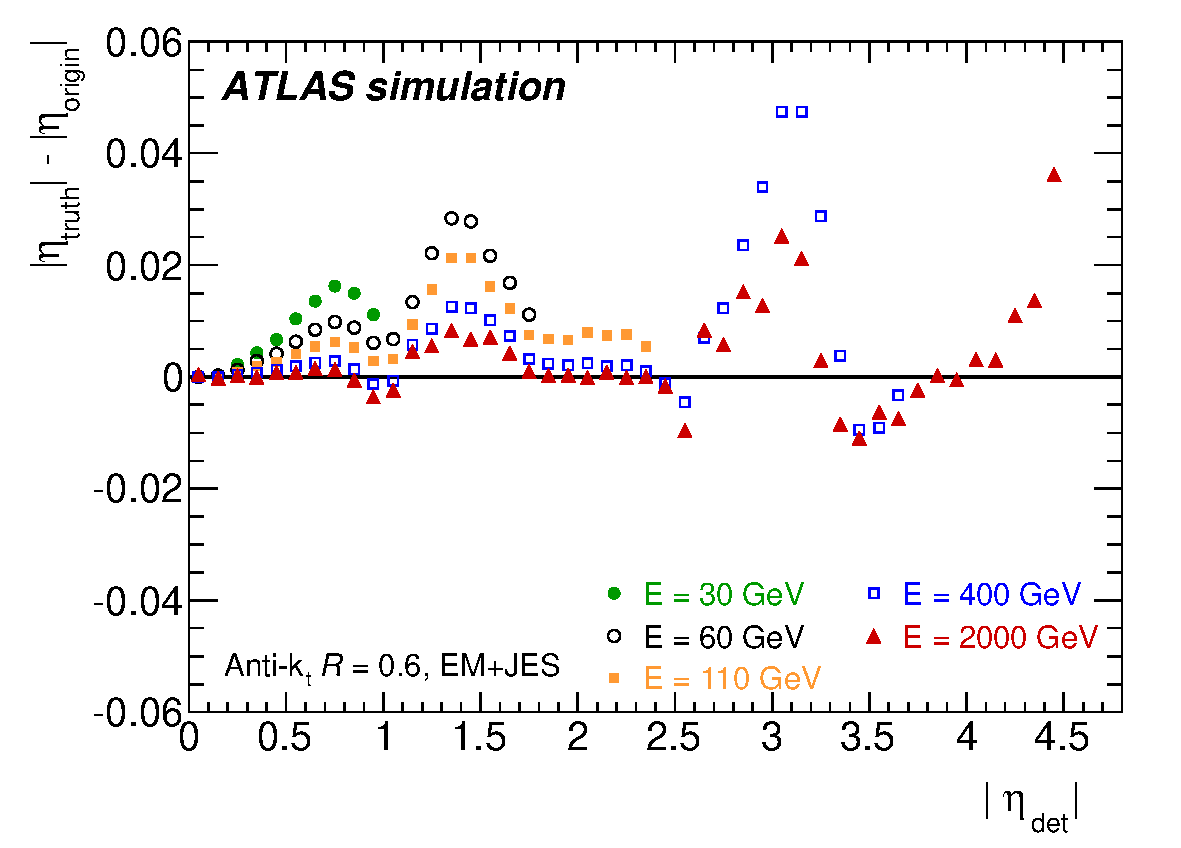
\includegraphics[width=0.6\textwidth]{total_eta.pdf}
\label{fig:jet-reconstruction:total-eta}
\caption{The full size of the $\eta$ calibration corrections, for different bins of energy and as a function of the detector $\eta$, for $R=0.6$ EM jets in 2010.}
\end{figure}

%%%%%%%%%%%%%%%% 

% If you bin in reco, you match truth to your reco jet. because your smaple has a a pt spectrum, you will match more low truth than high truth (though calorimter response means that you will have both up and down). this is a bias. if you bin in truth, the fluctuation up and down will be equal-- the calorimeter response will be the only thing causing up/down. thus, if your correction is binned in truth, it will not be biased, but it requires a numerical inversion to do correctly.


\subsection{Global Sequential Calibration}

Jets are calibrated to the particle scale in an inclusive dijet sample, which has a particular quark/gluon composition. Due to their different showering and hadronization properties-- gluons first split to quarks, and therefore typically have higher (but softer) particle multiplicities-- quark and gluon jets will have a different response in the detector. The Global Sequential Calibration of jets, following the JES, is a correction which uses measurable properties of jets to reduce this sensitivity to different types of hadronization, and therefore to quark/gluon flavor induced miscalibration~\cite{ATLAS-GSC}. Moreover, even jets of a single flavor type can fragment in wildly different ways, resulting in a range of possible responses: by measuring global jet properties, it is possible to better understand this fragmentation and correct the response jet-by-jet and thereby substantially improve the jet resolution.

Five variables are used to correct the jets; most of the variables are only available in some subset of the detector $\eta$. As the name of the technique suggests, these corrections are applied independently and sequentially. In order, these are:

\begin{enumerate}
	\item In $0 < |\eta| < 1.7$, $f_{\mathrm{Tile0}}$, the fraction of energy in the first layer of the tile calorimeter.
	\item In $0 < |\eta| < 3.5$, $f_{\mathrm{LAr3}}$, the fraction of energy in the third layer of the LAr EM calorimeter.
	\item In $0 < |\eta| < 2.5$, \ntrk, the number of primary-vertex tracks associated to a jet.
	\item In $0 < |\eta| < 2.5$, Track Width, the radial distribution of the $p_T$ of tracks associated to a jet, defined as:
	\begin{equation}
	\mathrm{Track~Width} = \frac{\sum_{i \in j} p_T^{i} \Delta R(i,j) }{\sum_{i \in j} p_T^i}
	\end{equation}
	where $i$ iterates over tracks associated to jet $j$.
	\item In $0 < |\eta| < 2.7$, $N_\mathrm{segments}$, the number of muon segments associated to a jet
\end{enumerate}
The first two variables, $f_{\mathrm{Tile0}}$ and $f_{\mathrm{LAr3}}$, measure the longitudinal shower profile of the jet. \ntrk measures the charged component of the jet fragmentation; the track width measures the shower profile in the $\eta-\phi$ plane. $N_{\mathrm{segments}}$ measures the amount of hadronic activity in the muon spectrometer, a result of so-called ``punch-through'' wherein not all hadrons are stopped and sampled by the calorimeters. Because LC jets already contain longitudinal information in the topo-clusters, the first two variables are ommitted for the GSC for that class of jets. Figure~\ref{fig:jet-reconstruction:gsc} shows the dependence of the jet response on these variables. The correction, as a function of the variable $x$, is defined as $C(x) = \mathcal{R}^{-1}(x)$, where $\mathcal{R}$ is the \pt response. This correction is binned finely in both \pt and $\eta$, and is normalized such that the inclusive response does not change. After the calibrations, the average response is 1 when measured by any of these variables, indicating that the jet energy measurement variance has been substantially reduced. Figure~\ref{fig:jet-reconstruction:resolution_gsc} shows the improvement in the \textit{jet resolution} (i.e., the width of a response measurement) as a function of \pt; the lower values after the GS correction, in blue, compared to the nominal in black, indicate that fluctuations in jet measurement have been reduced.


\begin{figure}
\centering
\subfigure[$f_{\mathrm{Tile0}}$]{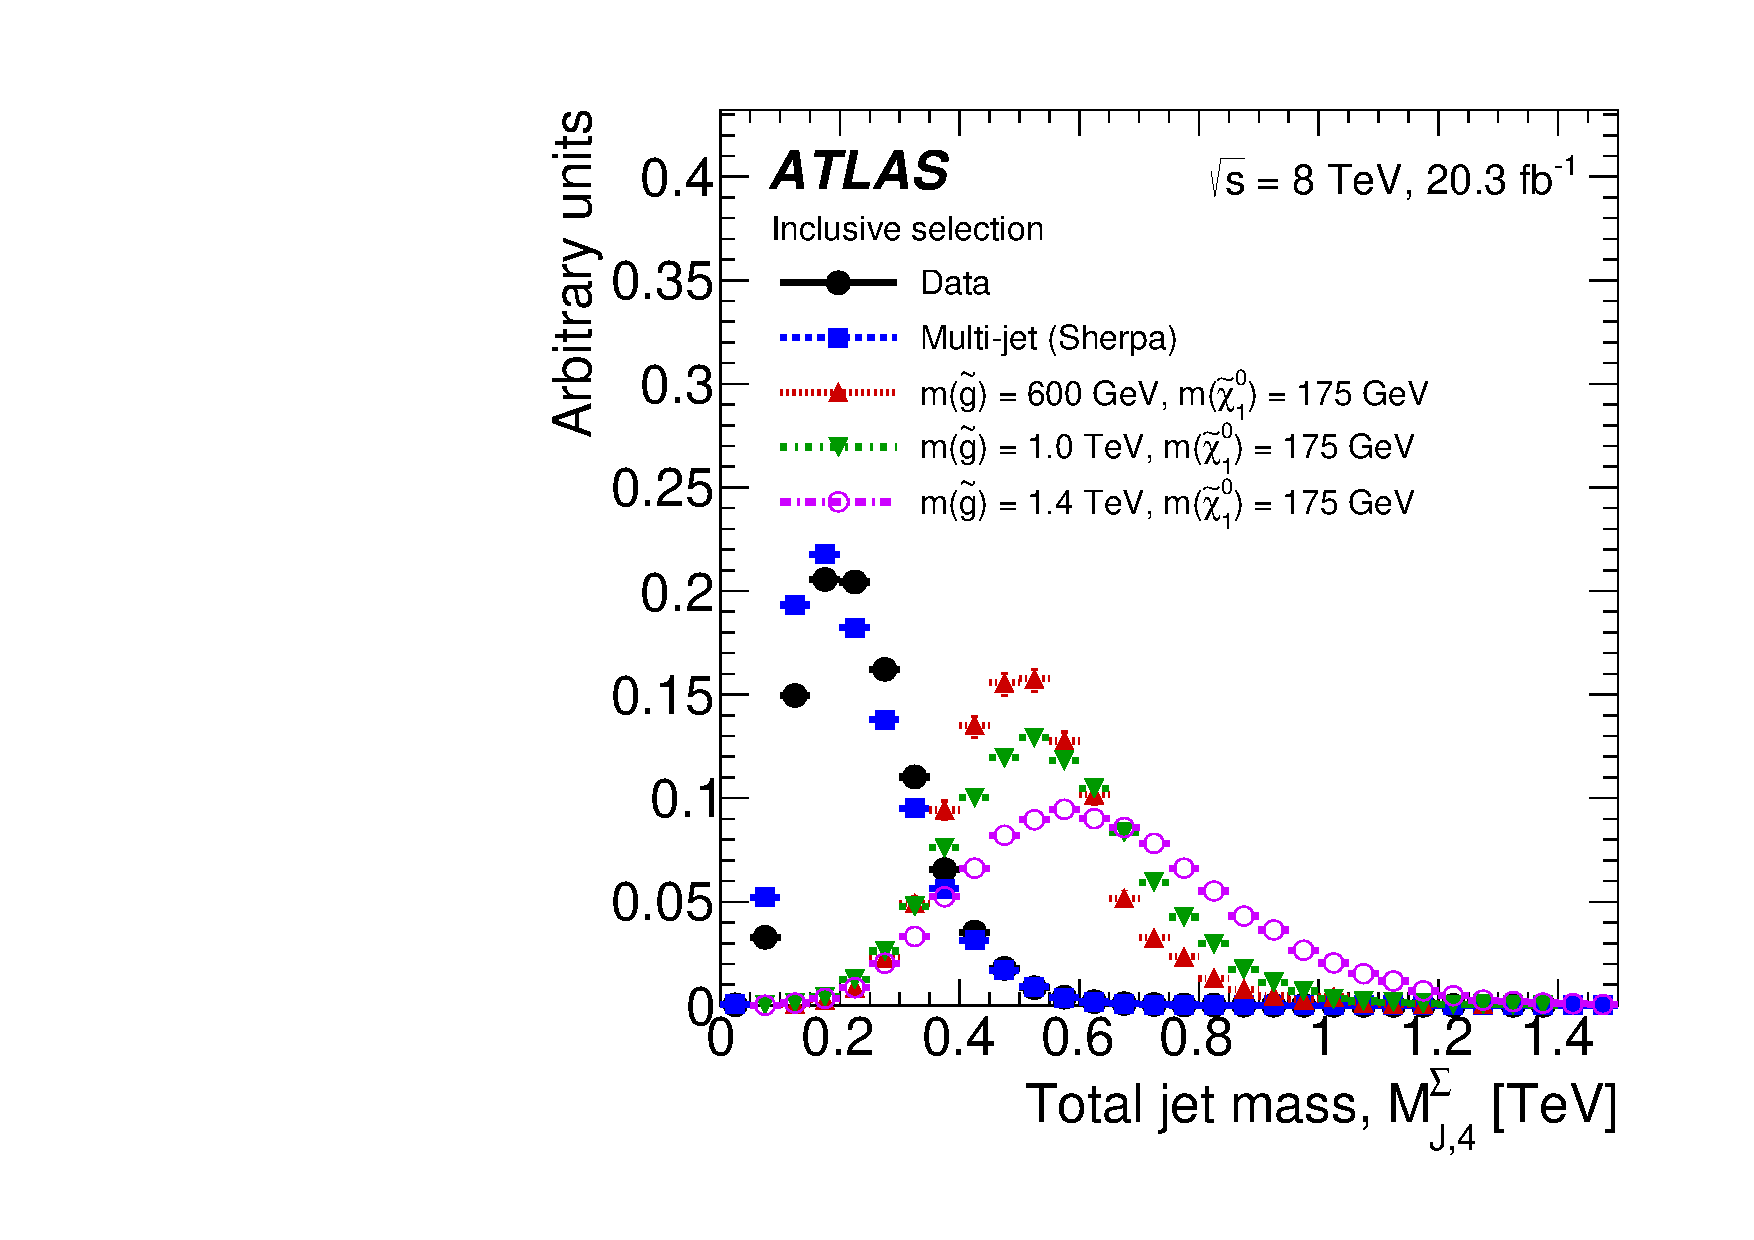
\includegraphics[width=0.3\textwidth]{fig_06a.pdf}}
\subfigure[$f_{\mathrm{LAr3}}$]{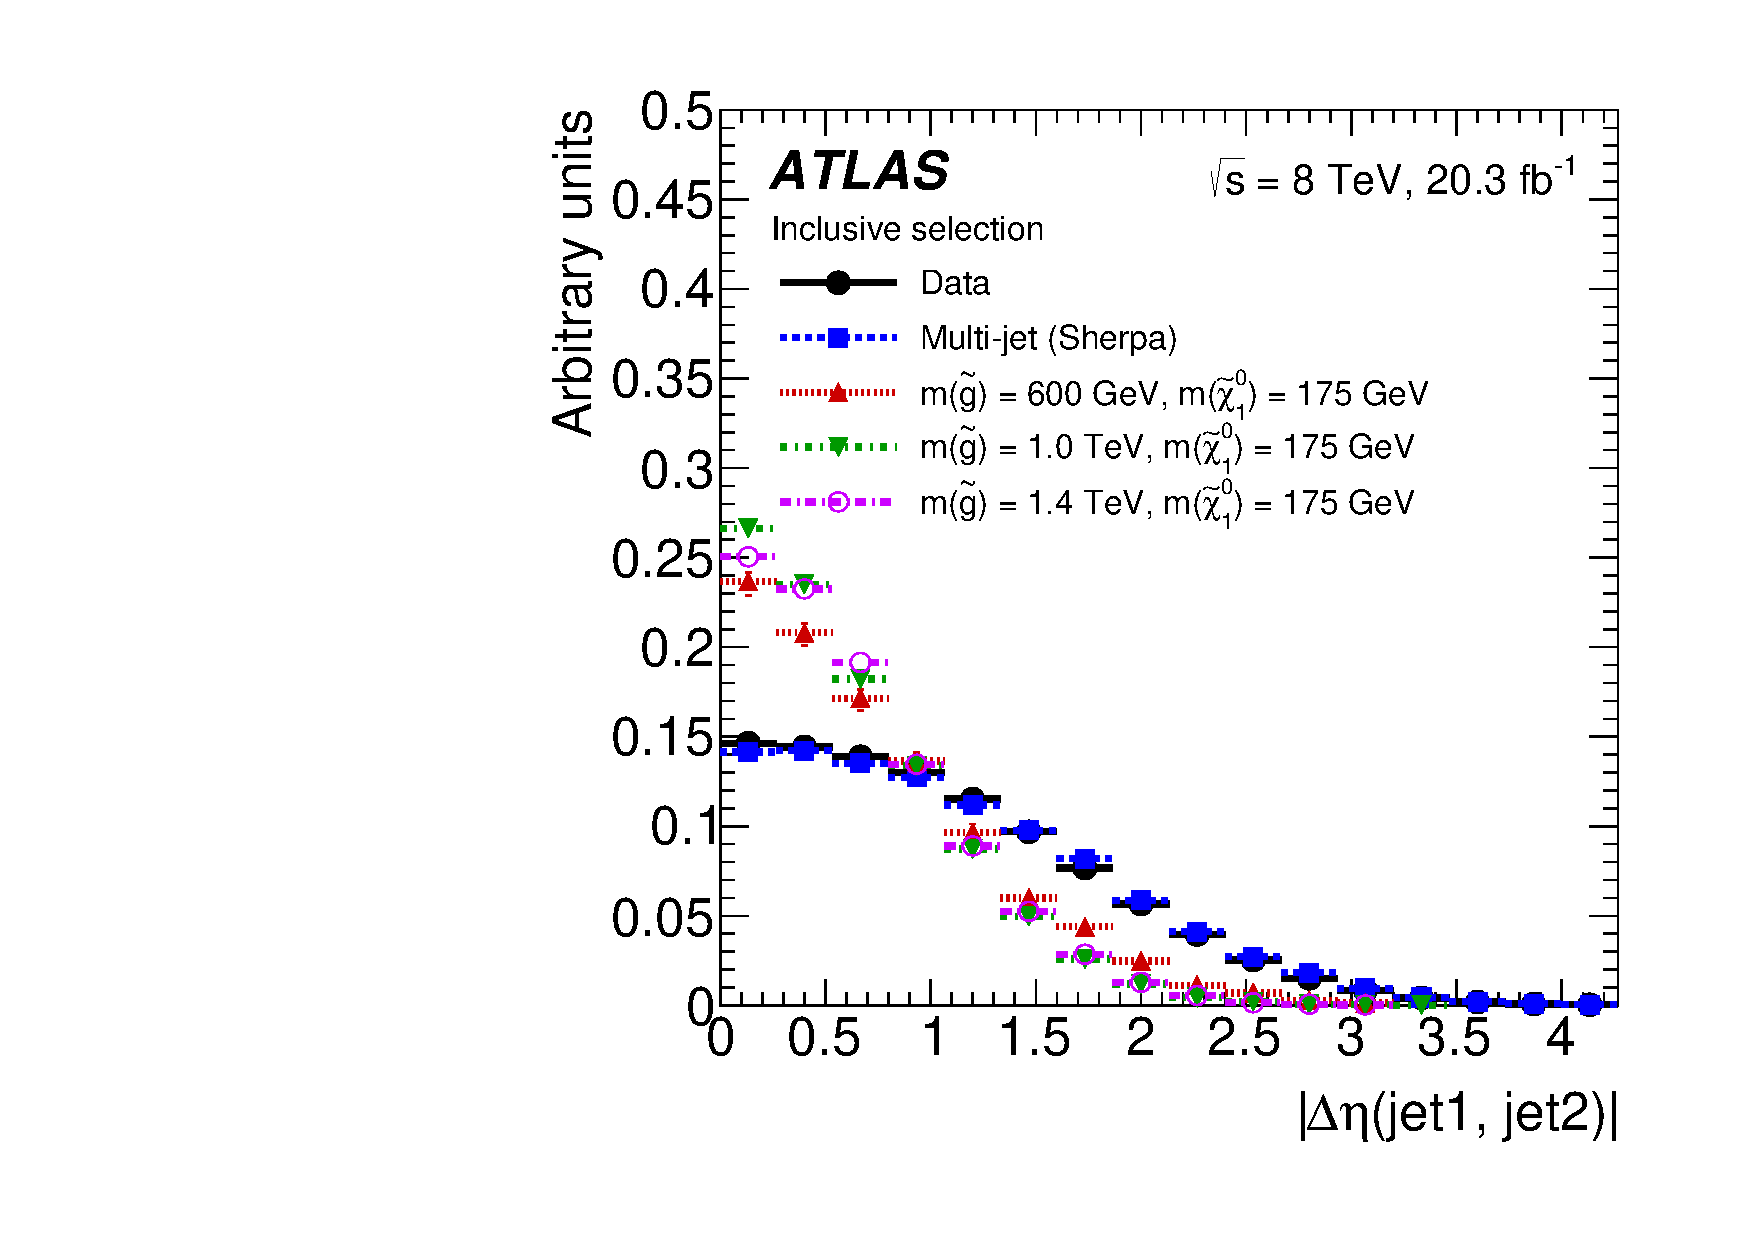
\includegraphics[width=0.3\textwidth]{fig_06b.pdf}}
\subfigure[\ntrk]{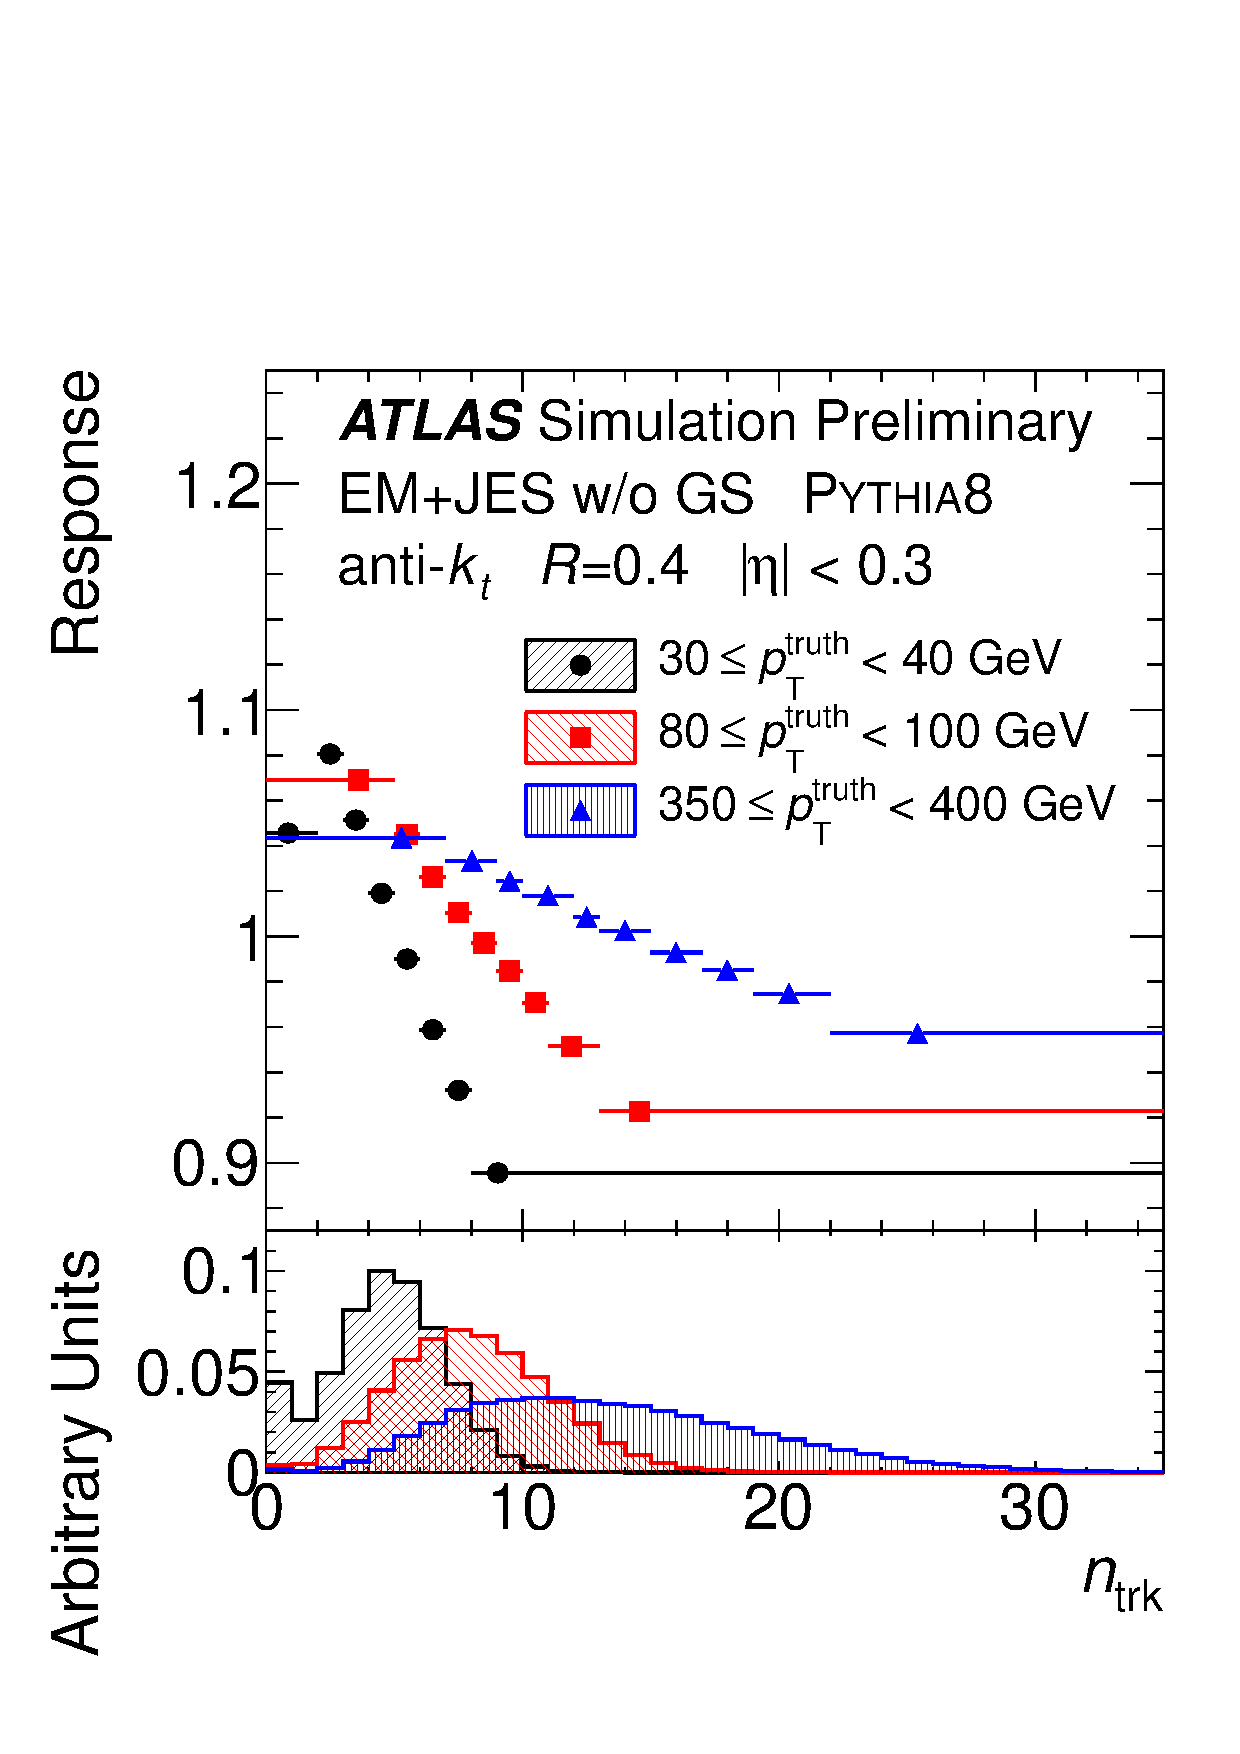
\includegraphics[width=0.3\textwidth]{fig_06c.pdf}}

\subfigure[Track Width]{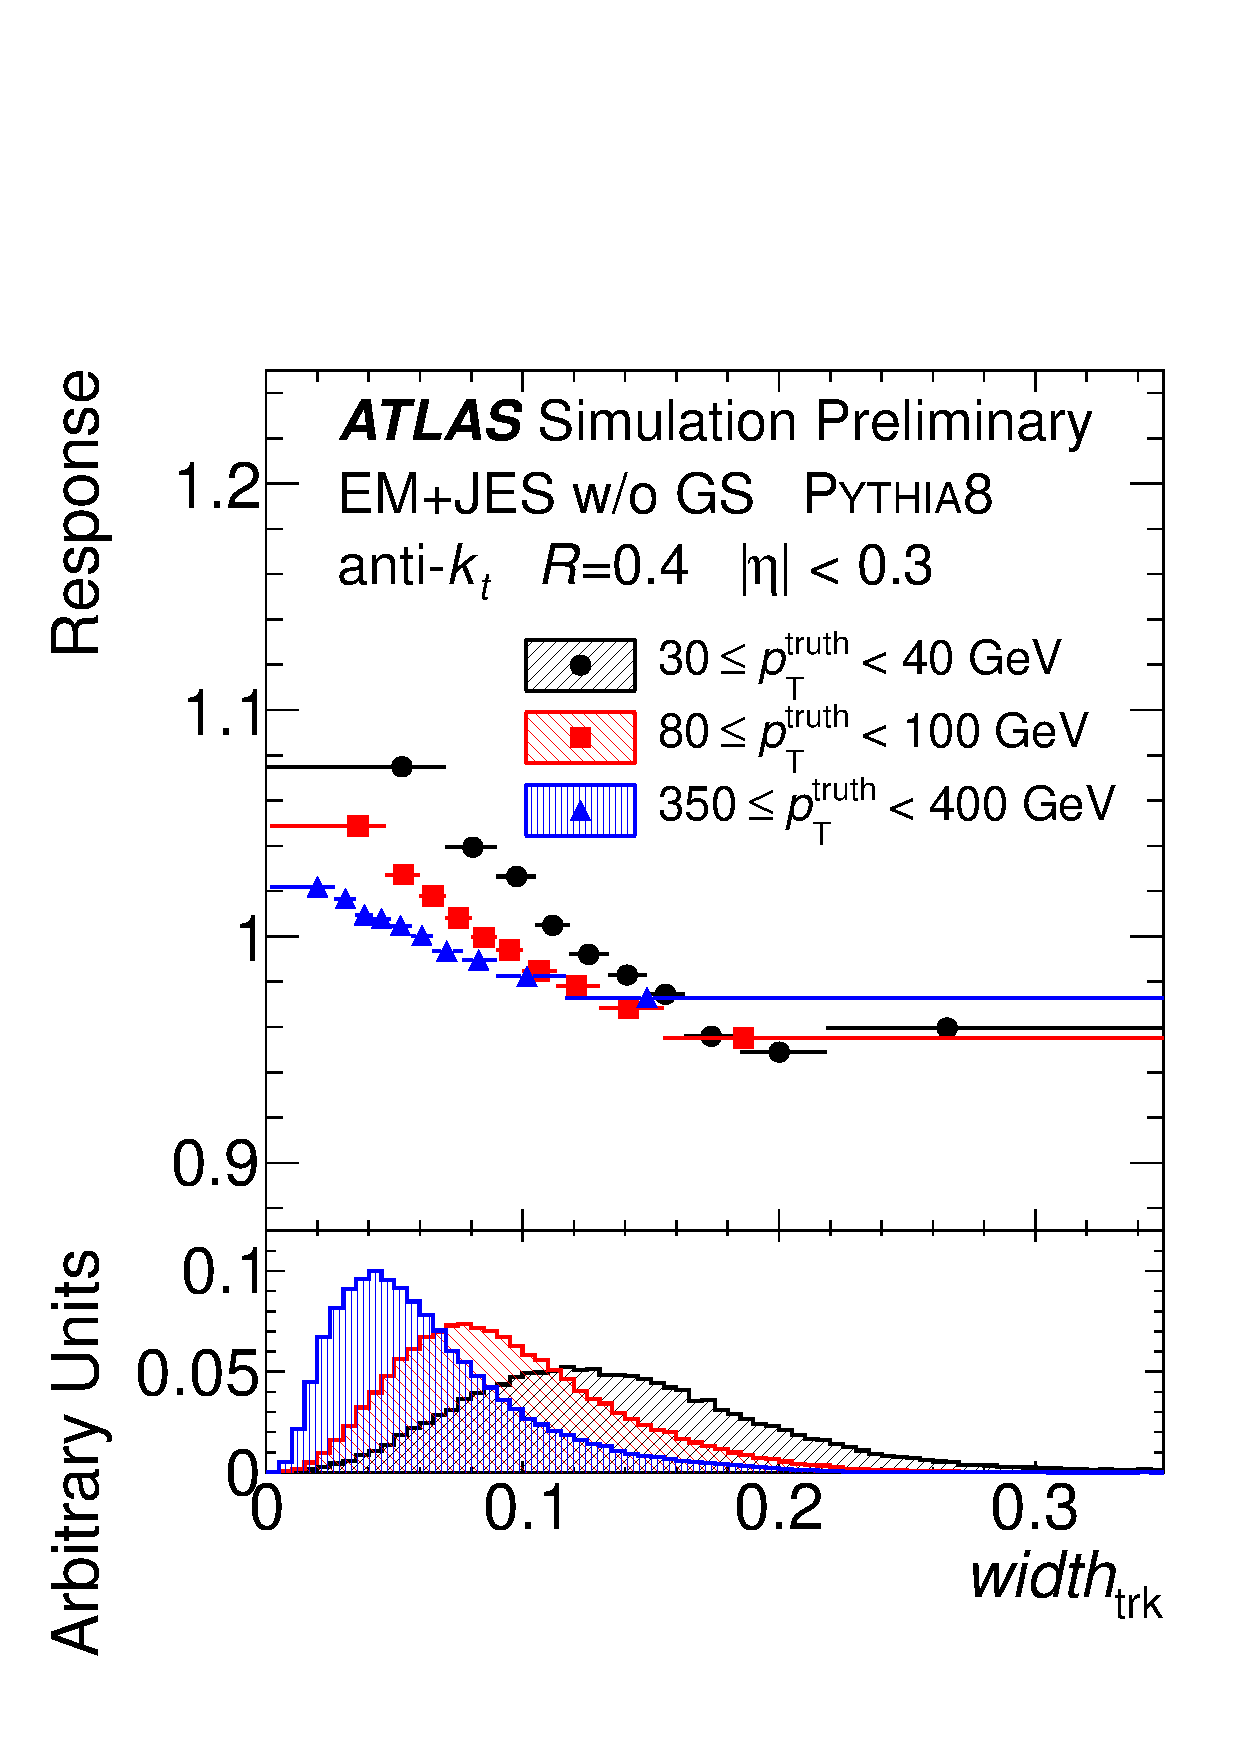
\includegraphics[width=0.3\textwidth]{fig_06d.pdf}}
\subfigure[$N_\mathrm{Segments}$]{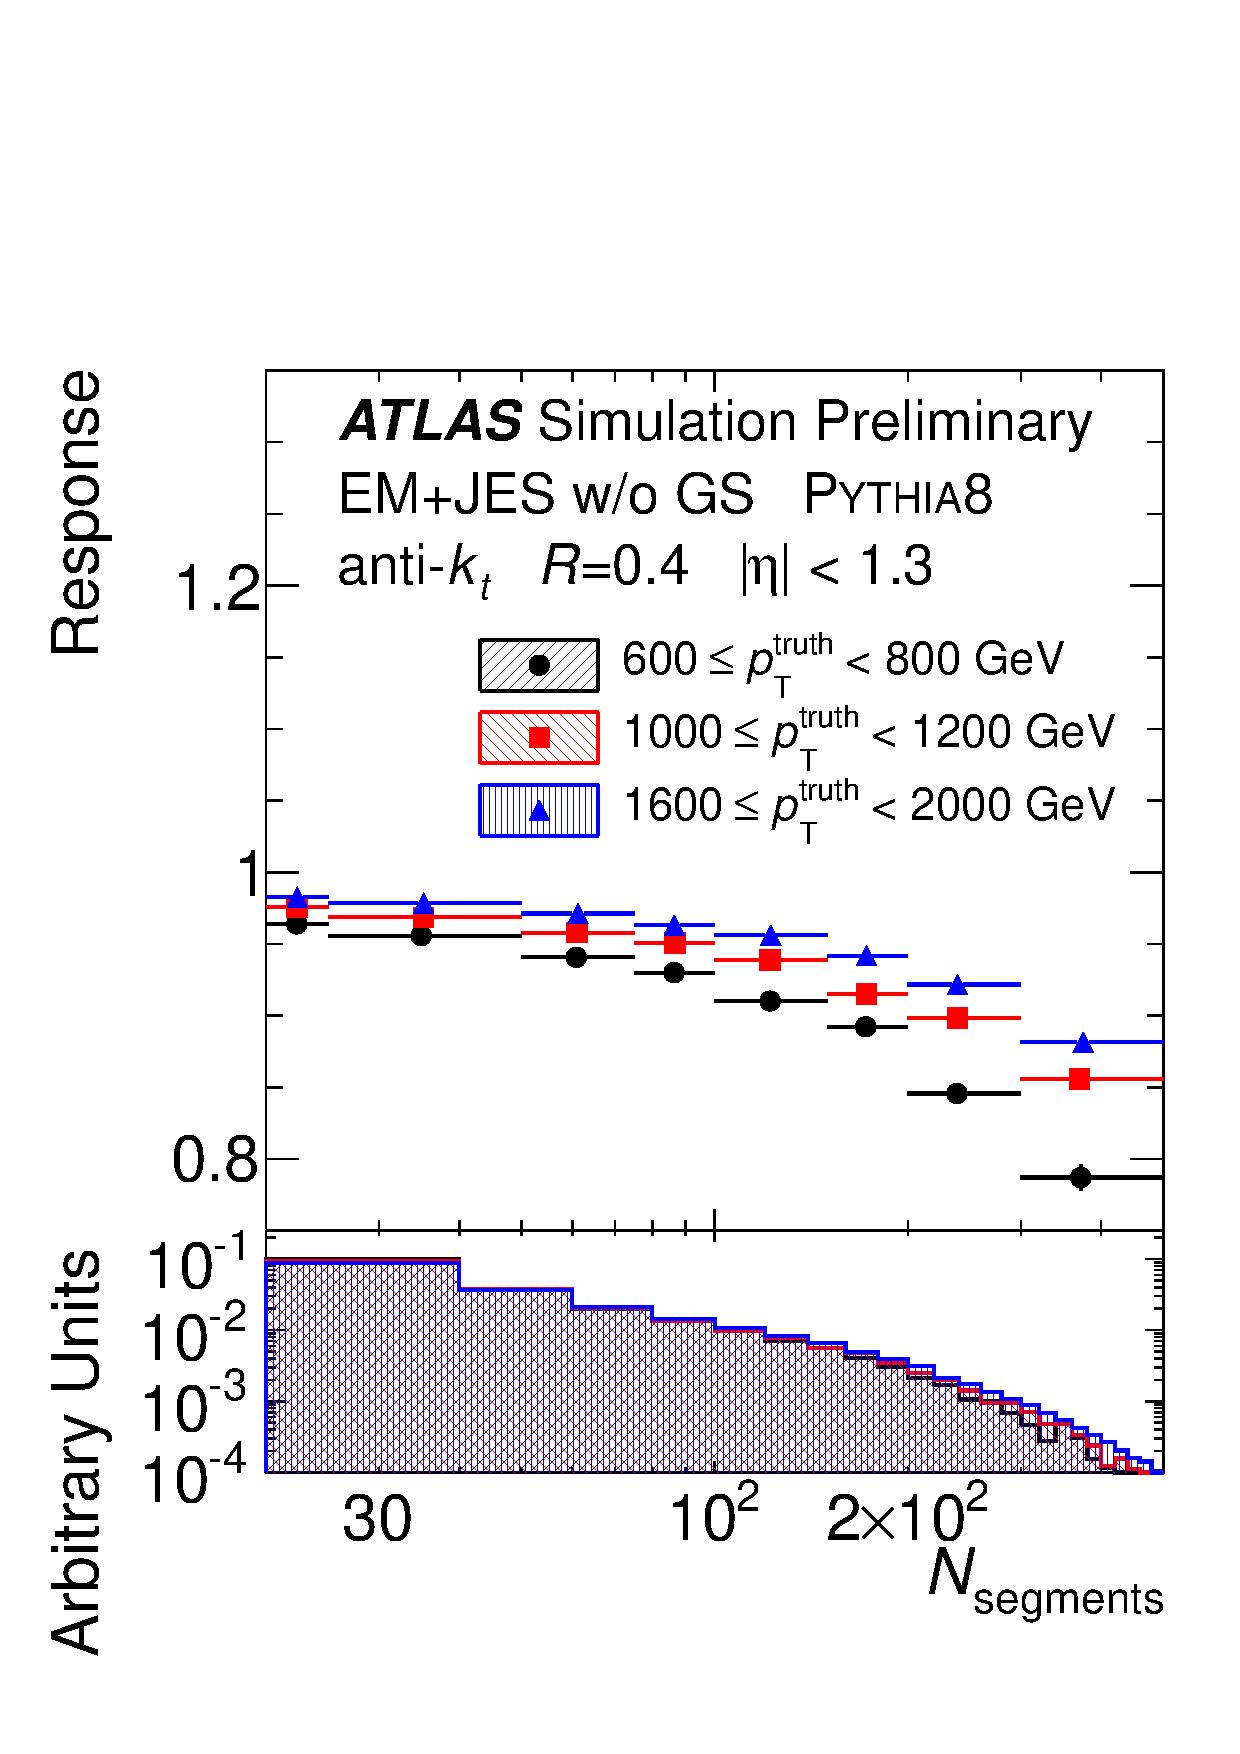
\includegraphics[width=0.3\textwidth]{fig_06e.pdf}}
\label{fig:jet-reconstruction:gsc}
\caption{The average jet response, as a function of each GSC variable, in a central bin of jet $\eta$.}
\end{figure}

\begin{figure}
\centering
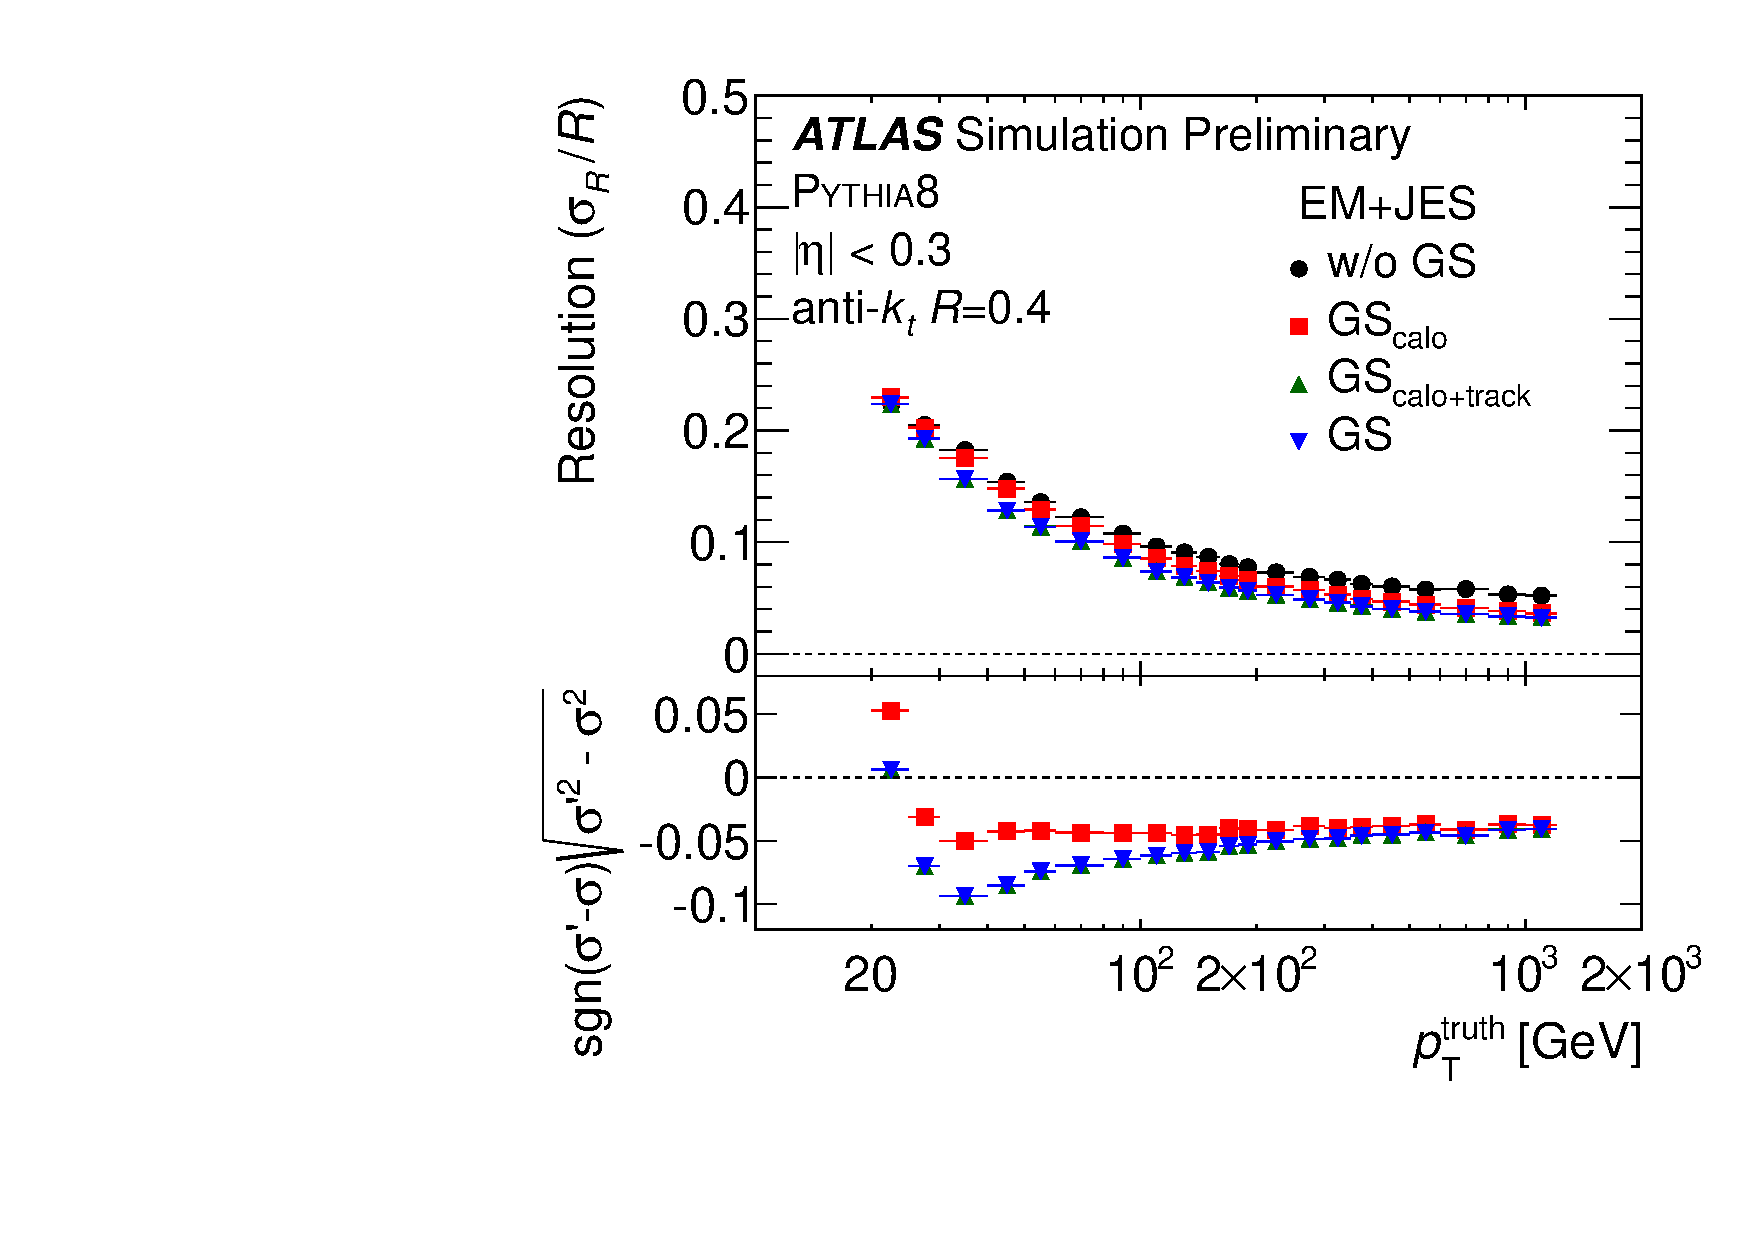
\includegraphics[width=0.6\textwidth]{fig_04a.pdf}
\label{fig:jet-reconstruction:resolution_gsc}
\caption{The improvement in jet resolution after applying the GSC correction.}
\end{figure}


\subsection{In-situ Calibrations}

Following the JES and GSC calibration steps, a final data-driven \textit{in-situ} calibration uses different jet balance techniques in data to develop a small residual correction and a measurement of the uncertainties on the final jet $p_T$ scale. $Z$+jet, $\gamma$+jet, and multi-jet measurements are used in low $p_T$, medium $p_T$, and high $p_T$ regions respectively.

In $Z$+jet measurements, a well reconstructed $Z$-boson, decaying in either the $e^+/e^-$ or $\mu^+/\mu^-$ channel, is used as a reference object to probe the quality of the jet energy measurement. In particular, a reference \pt is defined as $p_T^\mathrm{ref} = p_T^\mathrm{Z} \times |\cos(\mathrm{jet}, Z) |$ in order to take into account the potential presence of additional parton radiation which might affect the direct balance of the $Z$ and the leading jet. The mean of the response (defined as $\mathcal{R}_Z = p_T^\mathrm{jet} / p_T^\mathrm{ref}$) is measured using Poisson fits at low $p_T^\mathrm{ref}$ (due to inefficiency of the trigger cutting off the low end of the response) and the arithmetic mean at higher values; the disagreement between data and MC, as a function of $p_T^\mathrm{ref}$, is used to estimate the systematic uncertainty on the jet $p_T$. Figure~\ref{fig:jet-reconstruction:z_jet} shows an example of one such fit in a bin of $p_T^\mathrm{ref}$, and of the evolution of $\mathcal{R}_Z$ as a function of $p_T^\mathrm{ref}$.

%%%%%%%%%%%%%%%%

\begin{figure}
\centering
\subfigure[Example of a fit used to estimate $\mathcal{R}_Z$]{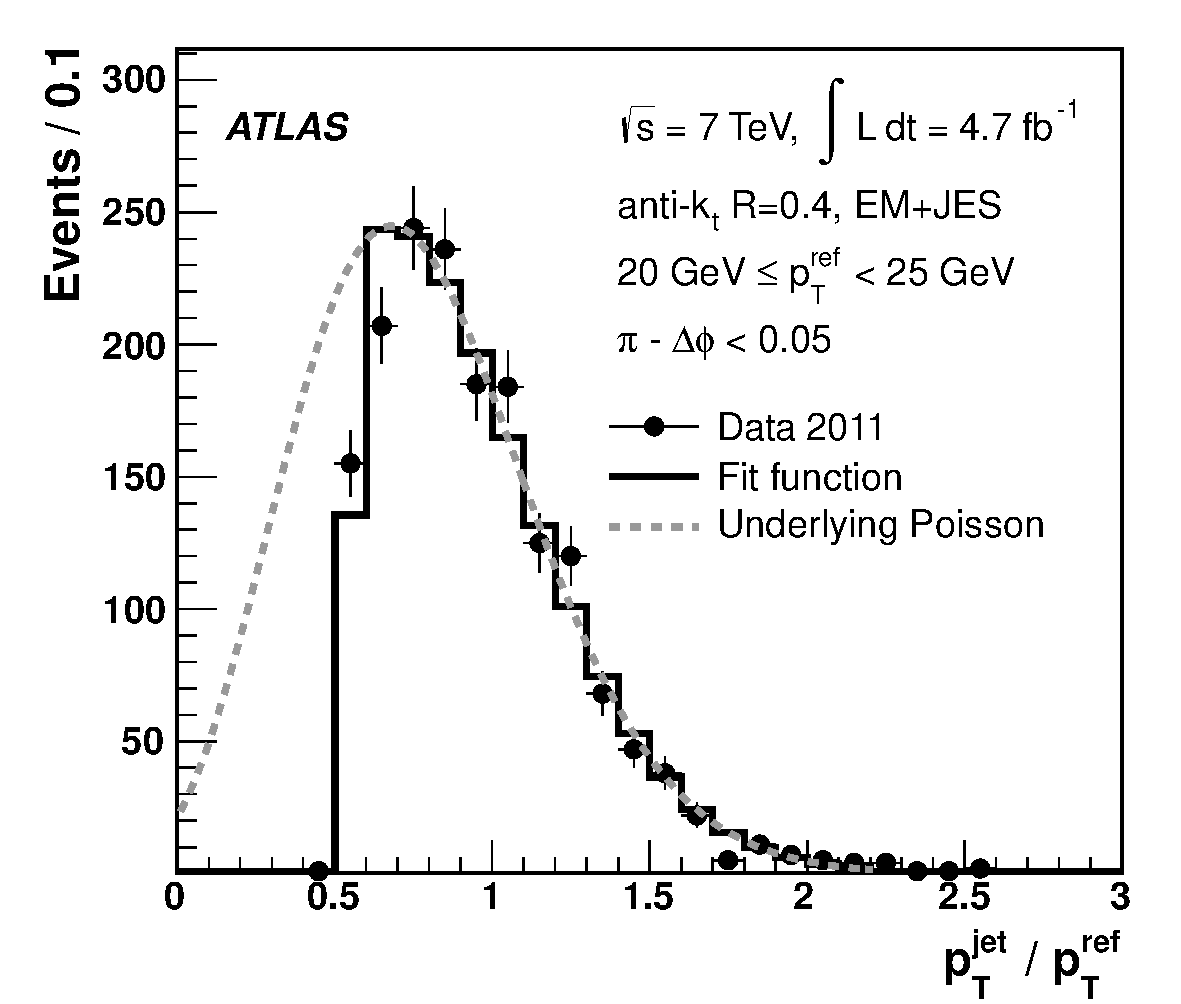
\includegraphics[width=0.45\textwidth]{fig_15a.pdf}}
\subfigure[Data/MC as a function of $p_T^\mathrm{ref}$]{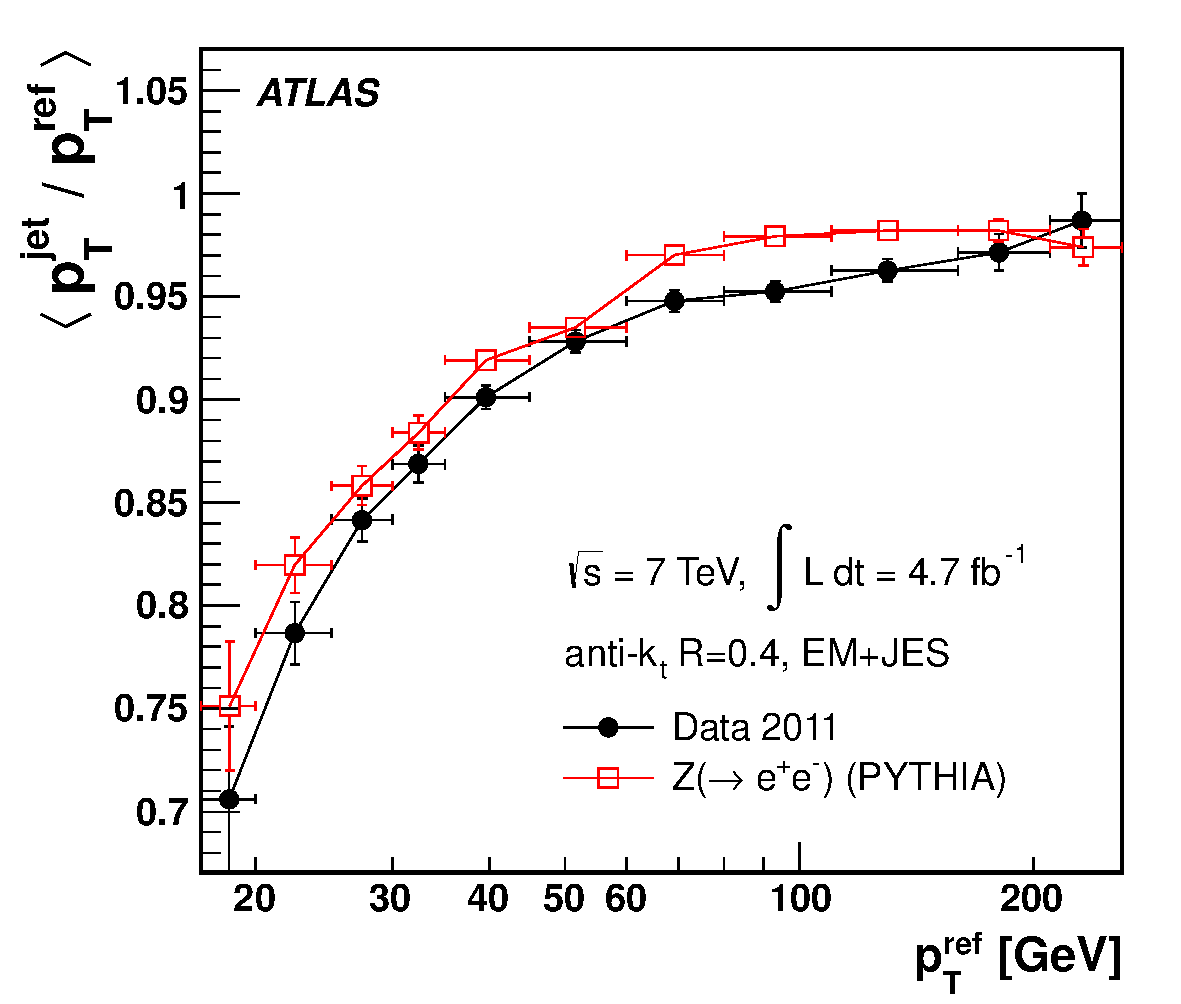
\includegraphics[width=0.45\textwidth]{fig_17a.pdf}}
\label{fig:jet-reconstruction:z_jet}
\caption{Examples of the measurements used to measure the uncertainties in jet $p_T$ at low \pt using $Z$+jet events.}
\end{figure}

%%%%%%%%%%%%%%%% 

The $\gamma$+jet measurements use a similar principle, and measures $\mathcal{R}_\gamma = p_T^\mathrm{jet} / p_T^\gamma$. High quality photon events are selected in both data and MC, and the $\mathcal{R}_\gamma$ is measured in both in fine bins of \pt and $\eta$. Poisson fits are used at low \pt because of trigger turn-on issues, and the arithmetic mean is used at higher values, to estimate the average response as a function of $p_T^\gamma$.  Figure~\ref{fig:jet-reconstruction:gamma_jet} shows an example of a fit to $\mathcal{R}_\gamma$ in one bin of $p_T^\gamma$ and the evolution of the mean value as a function of $p_T^\gamma$.

%%%%%%%%%%%%%%%%

\begin{figure}
\centering
\subfigure[Example of a fit used to estimate $\mathcal{R}_\gamma$]{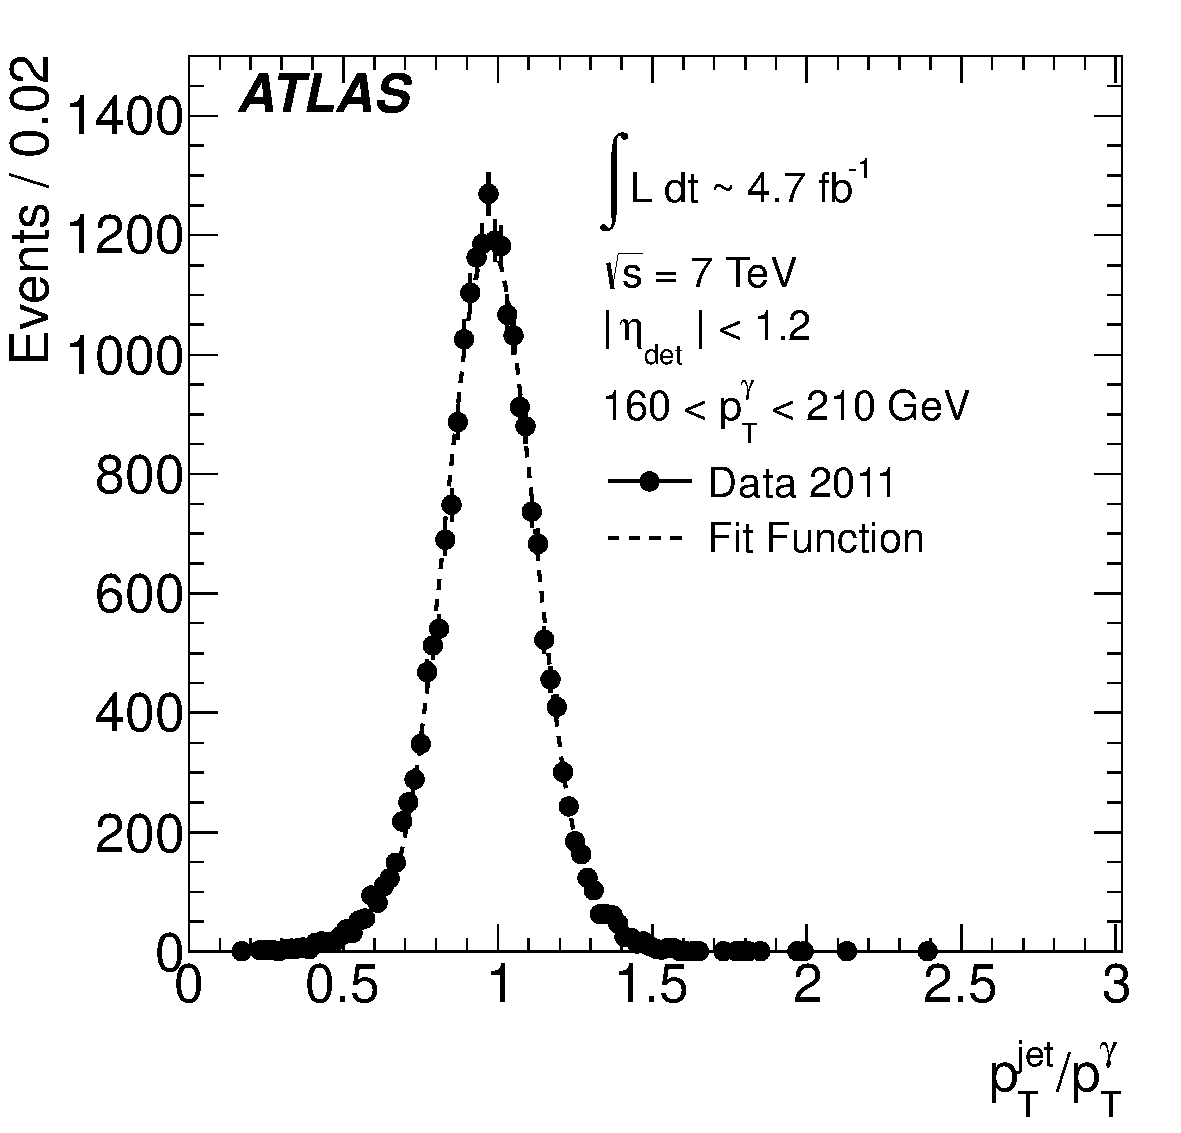
\includegraphics[width=0.45\textwidth]{fig_22b.pdf}}
\subfigure[Data/MC as a function of $p_T^\gamma$]{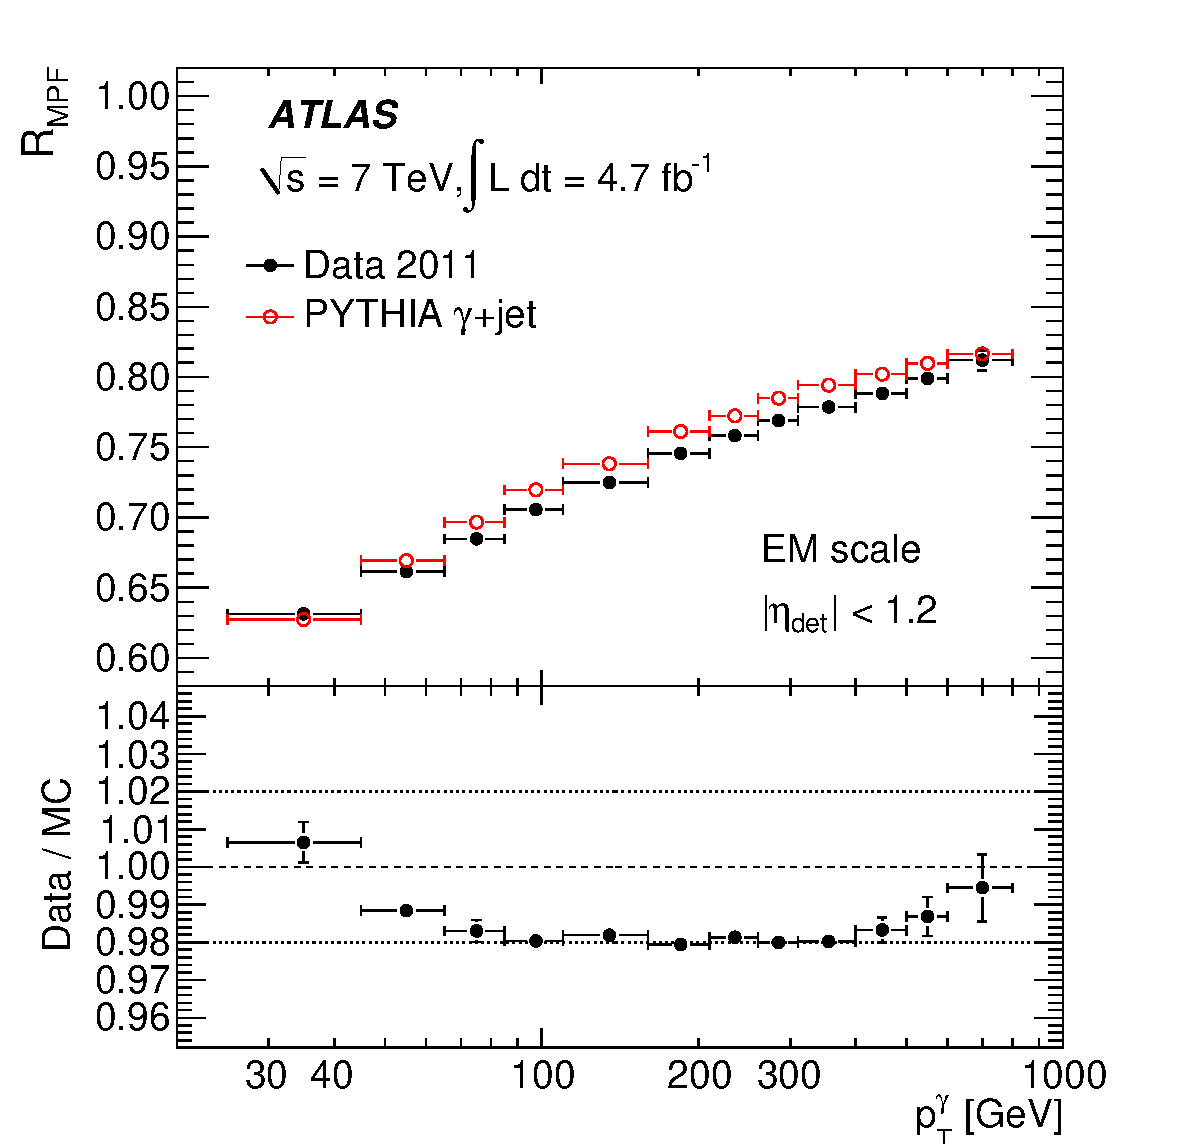
\includegraphics[width=0.45\textwidth]{fig_23a.pdf}}
\label{fig:jet-reconstruction:gamma_jet}
\caption{Examples of the measurements used to measure the uncertainties in jet $p_T$ at moderate \pt using $\gamma$+jet events.}
\end{figure}

%%%%%%%%%%%%%%%% 

At high \pt, a multijet balance technique is used to derive uncertainties. In this technique, a leading jet with \pt significantly higher than a system of low \pt jets is balanced against that system; the uncertainties on the well-measured low \pt jets are propagated in order to estimate the \pt of the leading jet. The multijet balance is defined as $\mathrm{MJB} = \frac{|\vec{p}_T^{\mathrm{jet}}|}{|\vec{p}_T^{\mathrm{recoil}}|} $; events used in the analysis are required to have $p_T^\mathrm{leading} < $


\subsection{\LargeR Calibrations}

The standard jet calibration chain is run only on $R=0.4$ and $R=0.6$ jets, using both LC and EM scale inputs. For analyses which require the use of jets with a different $R$ parameter and/or grooming, another set of calibrations must be performed. Optimization studies on a variety of signal classes in 2011 determined that the collection \antikt $R=1.0$ with trimming applied, using $\Rsub = 0.3$ and $\fcut = 0.05$, performed very well in a number of final states, and presented a very small susceptibility to pileup as demonstrated in Figure~\ref{fig:jet-reconstruction:pileup_large}~\cite{ATLAS-SS-2011}. This collection was thus centrally supported in 2012, and both calibrations and uncertainties were provided.

\begin{figure}
\centering
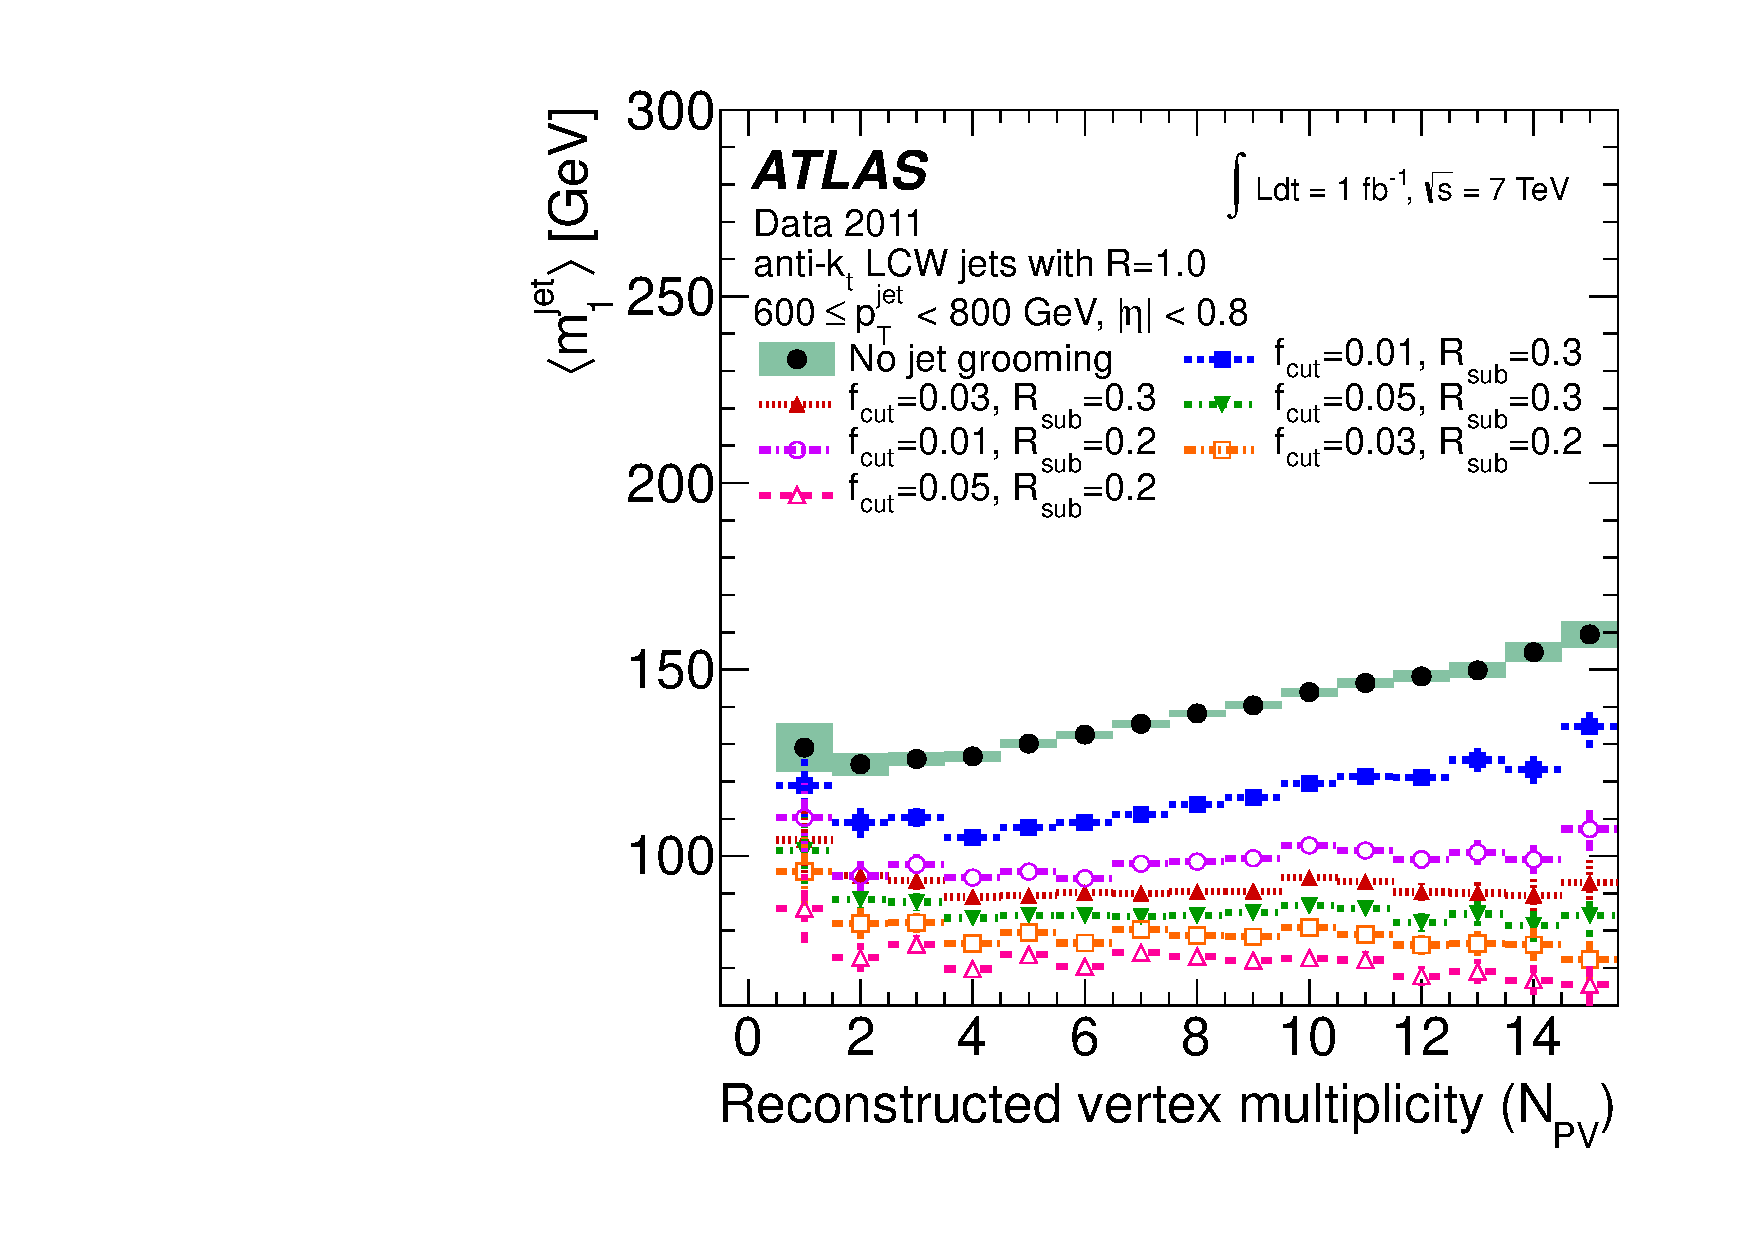
\includegraphics[width=0.6\textwidth]{fig_18b.pdf}
\label{fig:jet-reconstruction:pileup_large}
\caption{The dependence of the average lead jet mass in dijet events in 2011 data for ungroomed \antikt $R=1.0$ jets and several configurations of trimming.}
\end{figure}


The calibration procedure for these \largeR jets is slightly different than for the other collections. As most users are interested in the substructure properties of the jets, and using constituents at the hadron-scale is more sensible than the raw detector outputs, only LC inputs are used for \largeR jets. Additionally, because trimming effectively removes a large portion of the pileup contamination in the jets, no dedicated pileup correction procedure is applied (though in principle, it is possible to easily add an areas correction to the subjets before they are trimmed, and this should improve performance). This is visible in Figure, which shows the lack of sensitivity of the jet mass to additional pileup interactions. Thus, the MC JES procedure is performed on jets at the LC scale.

The MC JES procedure itself is identical to that described in Section~\ref{jet-reconstruction:jet-calibration-mc-jet-energy-scale}, except that an additional \textit{mass calibration} step is performed. This procedure defines a mass response in the typical way,
%
\begin{equation}
\mathcal{R}^{\mathrm{jet}}_m = m^{\mathrm{jet}}_{\mathrm{reco}} /  m^{\mathrm{jet}}_{\mathrm{truth}} 
\end{equation}
%
and performs a numerical inversion calibration procedure identical to the energy calibration procedure, after both the energy and $\eta$ are calibrated. This procedure is required because of the varying mass response of the calorimeter, as displayed in Figure~. This is again caused by the varying performance of detector technologies which change as a function of $\eta$: hadrons on one side of the jet, without a calibration, would cause more mass in the jet than the other side, even if they had the same energy. As the mass of \largeR jets is commonly used as a discriminating variable in analyses (as opposed to the $R=0.4$, which is rarely if ever used), it is important that the variable have a consistent meaning as the detector technology changes. Figure~\ref{fig:jet-reconstruction:total_jms} shows the effect of the jet calibration in 2011; while the mass response is close to $1$ in central $\eta$ bins, it can be substantially mismeasured at higher values of $\eta$ when the jet energy is low.

\begin{figure}
\centering
\subfigure[Before mass calibration]{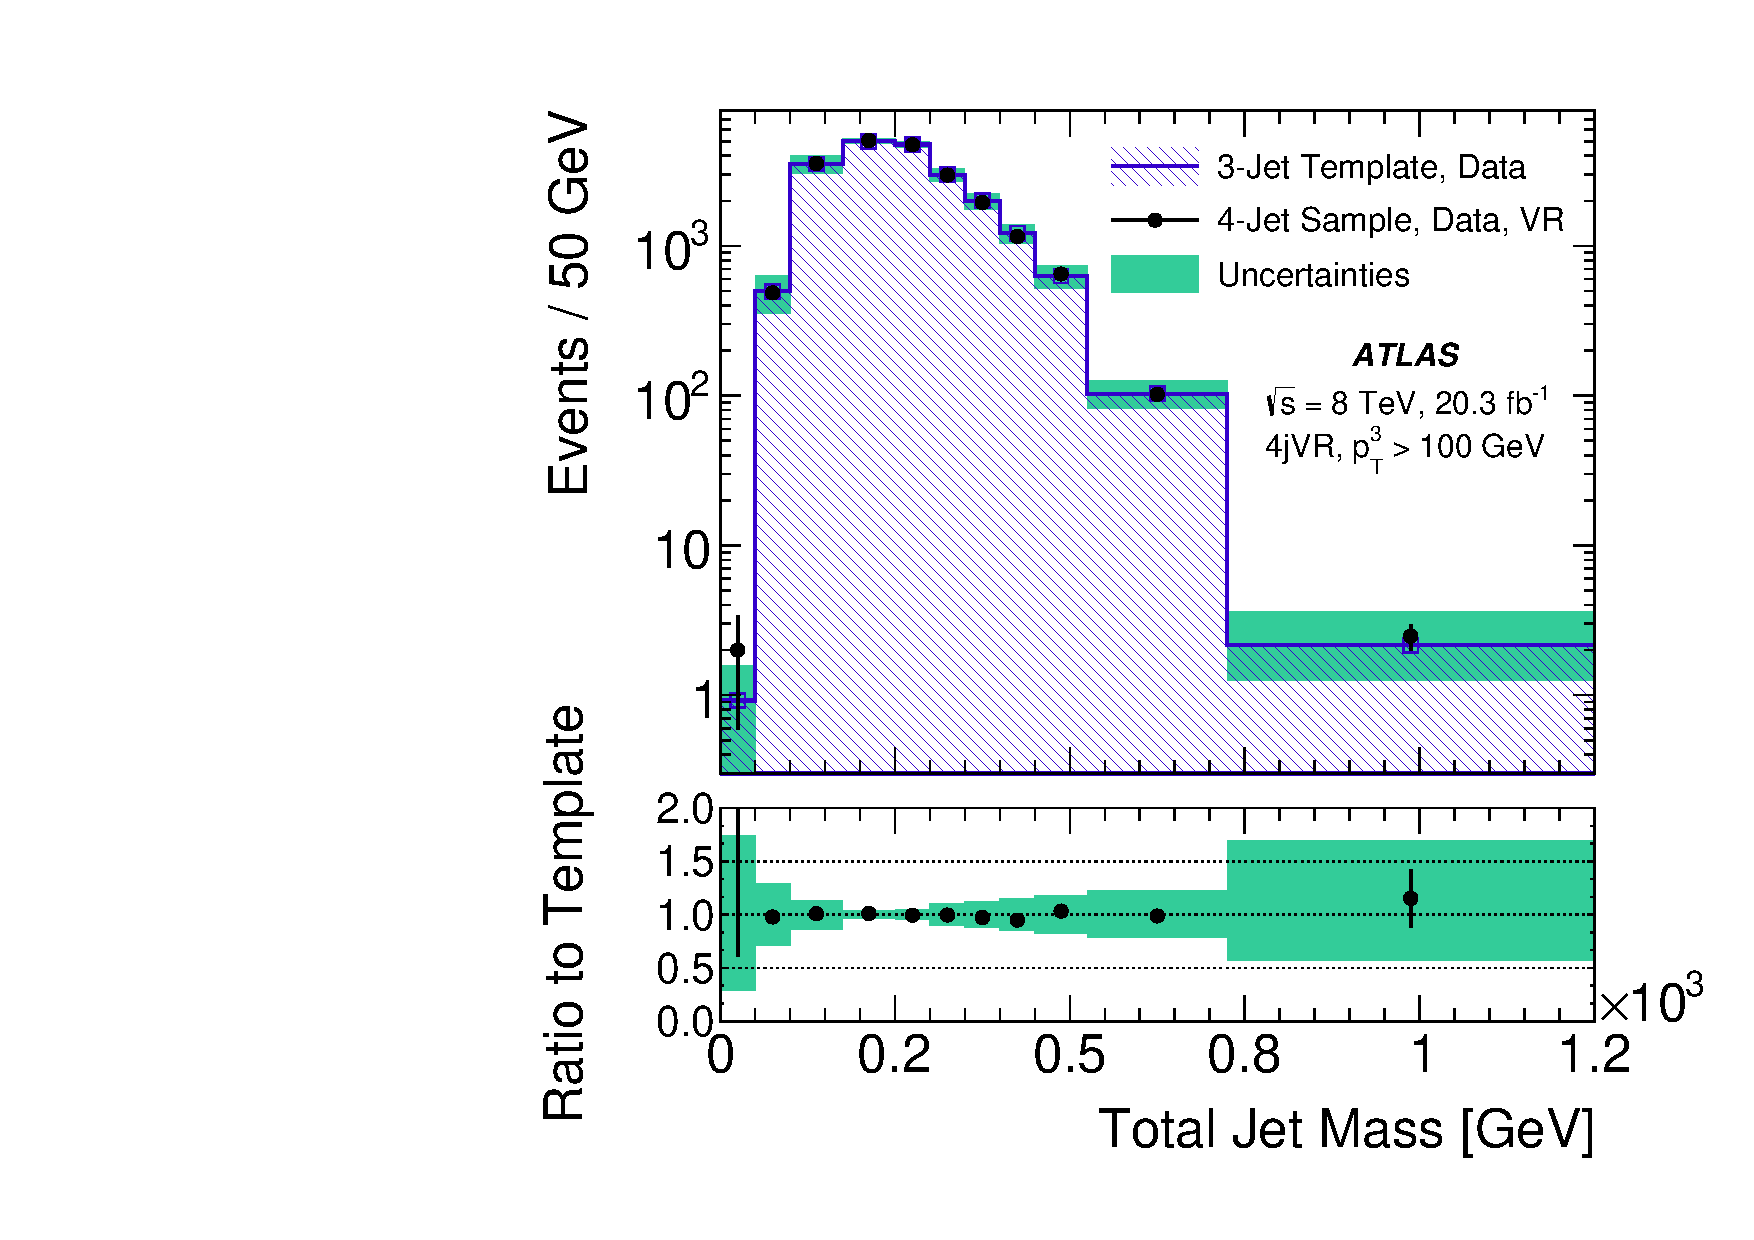
\includegraphics[width=0.45\textwidth]{fig_07a.pdf}}
\subfigure[After mass calibration]{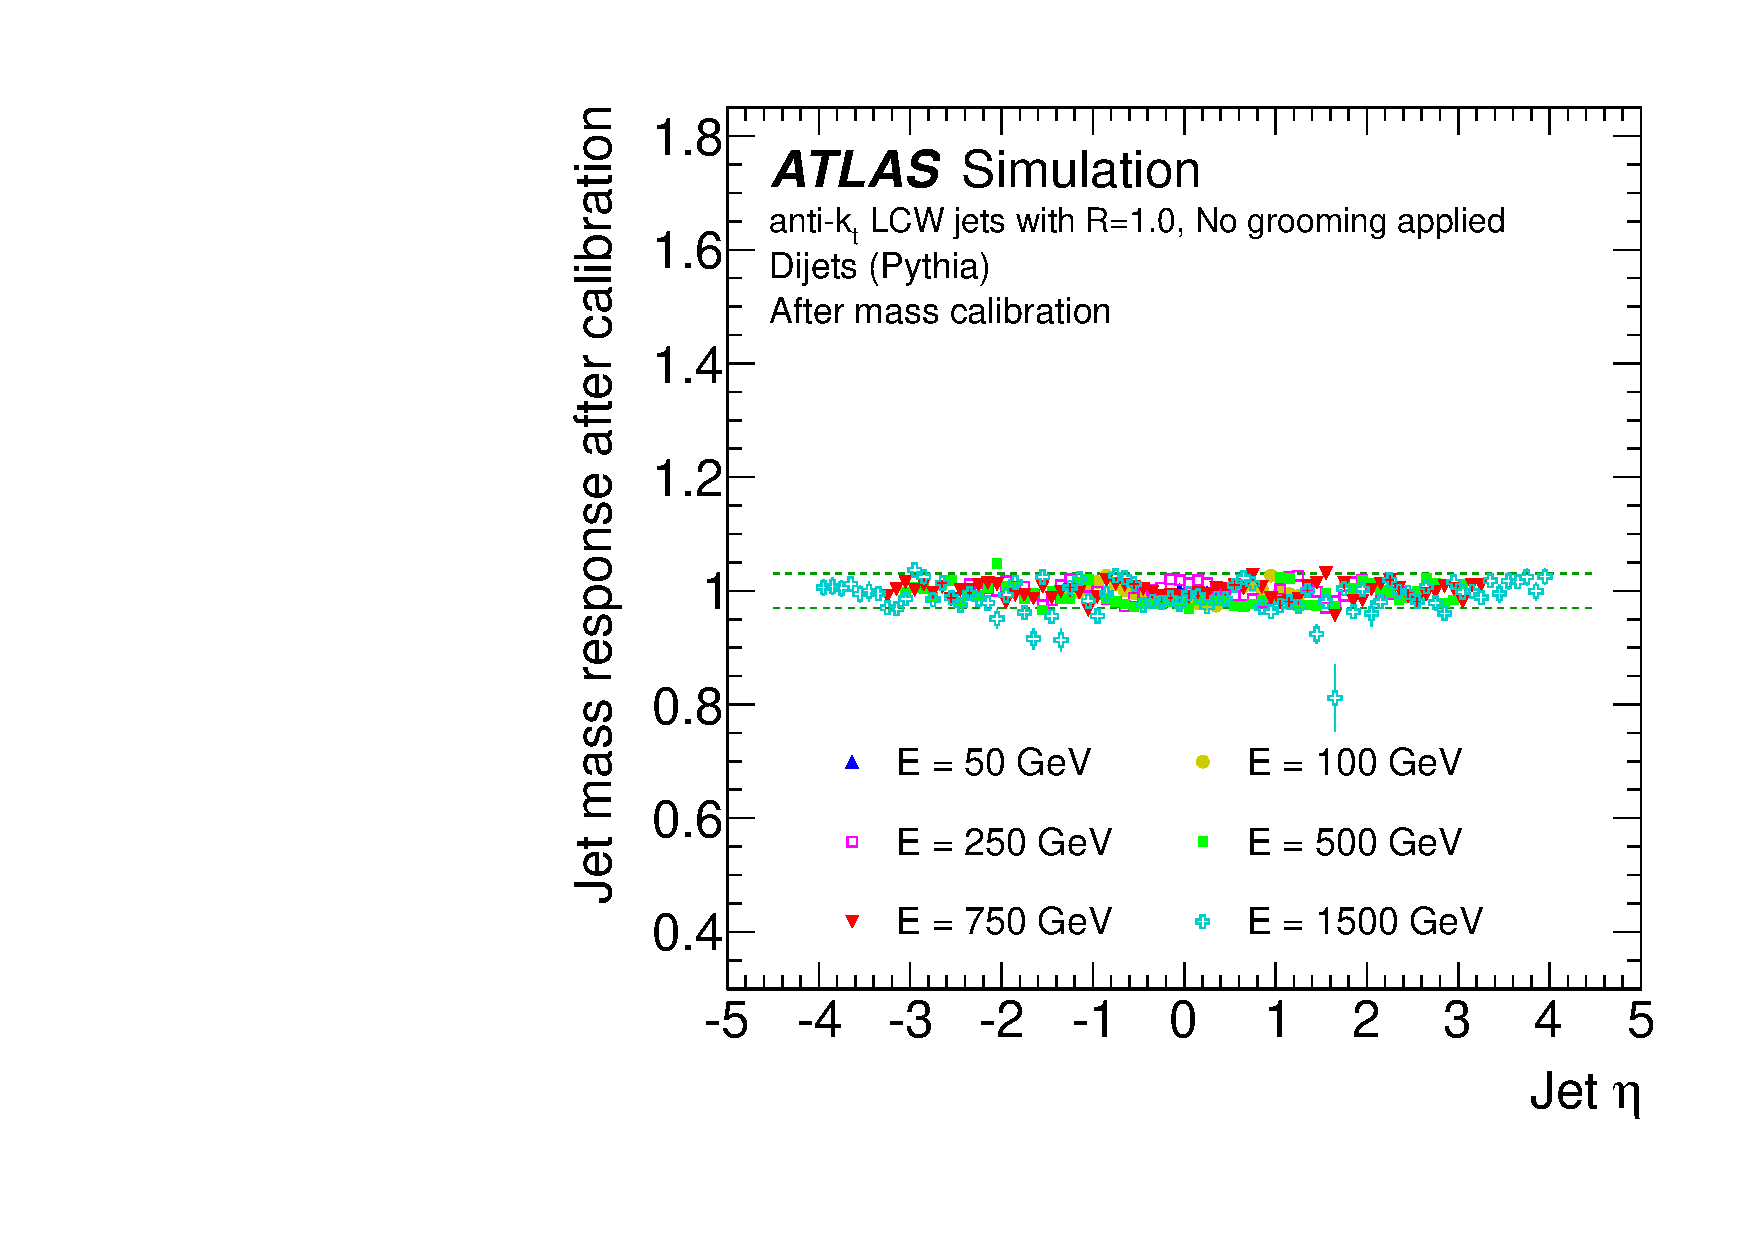
\includegraphics[width=0.45\textwidth]{fig_07b.pdf}}
\label{fig:jet-reconstruction:total_jms}
\caption{The mass response, for different bins of jet energy, as a function of jet $\eta$, before and after the calibration procedure.}
\end{figure}

Uncertainties on the \largeR jets are derived using a track-jet double ratio technique. Track-jets reconstructed with the same jet algorithm are matched to the calorimeter jets in a multi-jet sample, in both data and simulation. The ratio of the track-jet mass to the calorimeter mass is then measured: this provides a comparison of two indepenent measurements of the jet mass. The ratio of this ratio gives a bound on the disagreement of the modelling of the jet mass (or $p_T$, or other quantities) in the simulation.  These uncertainties, while conservative because of the introduction of charged fragmentation modeling, provide an \textit{in-situ} alternative measurement of the jet mass and other substructure properties. Figure~\ref{fig:jet-reconstruction:jms_uncertainty} shows both the raw track-to-calo mass ratio, and the corresponding derived uncertainty as a function of the jet \pt, in 2011 data.

\begin{figure}
\centering
\subfigure[Track/Calo Mass]{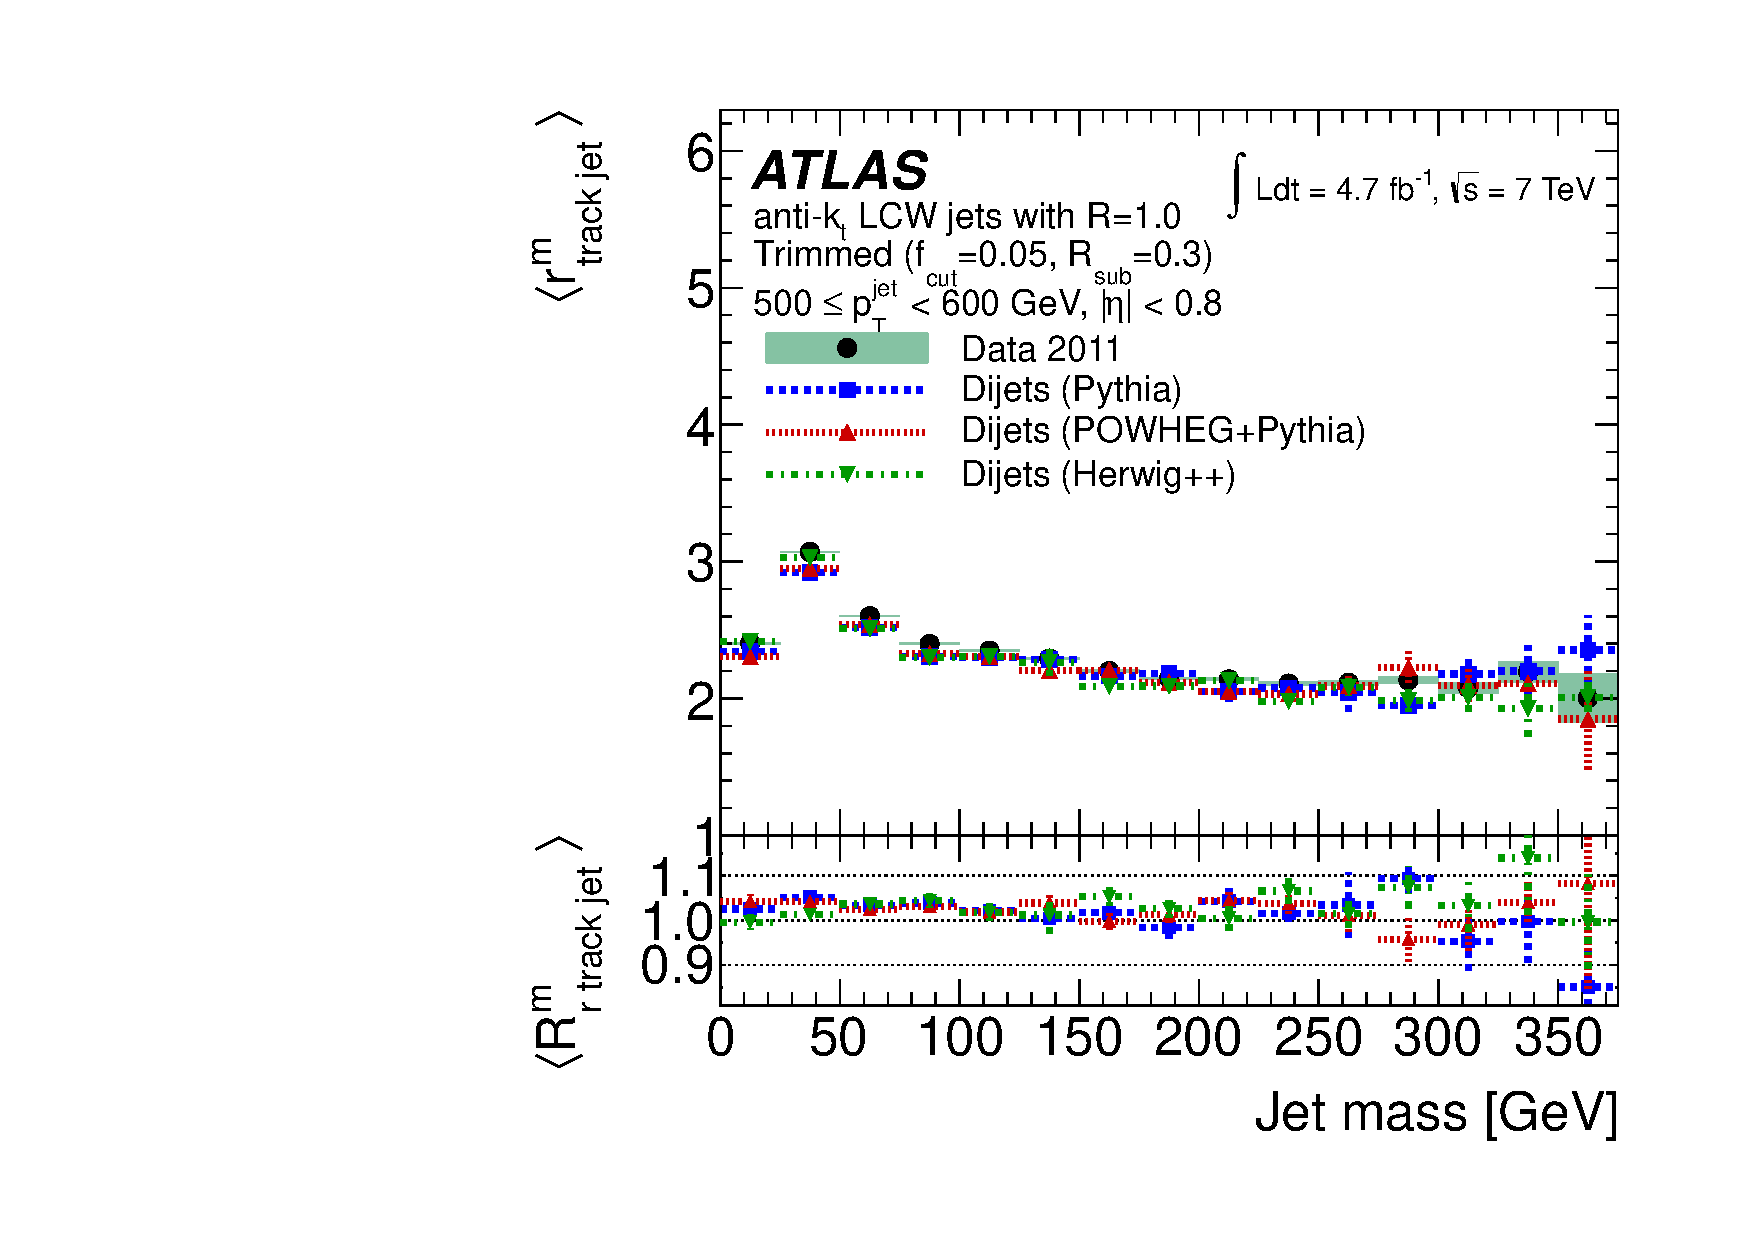
\includegraphics[width=0.45\textwidth]{fig_09b.pdf}}
\subfigure[Mass uncertainty]{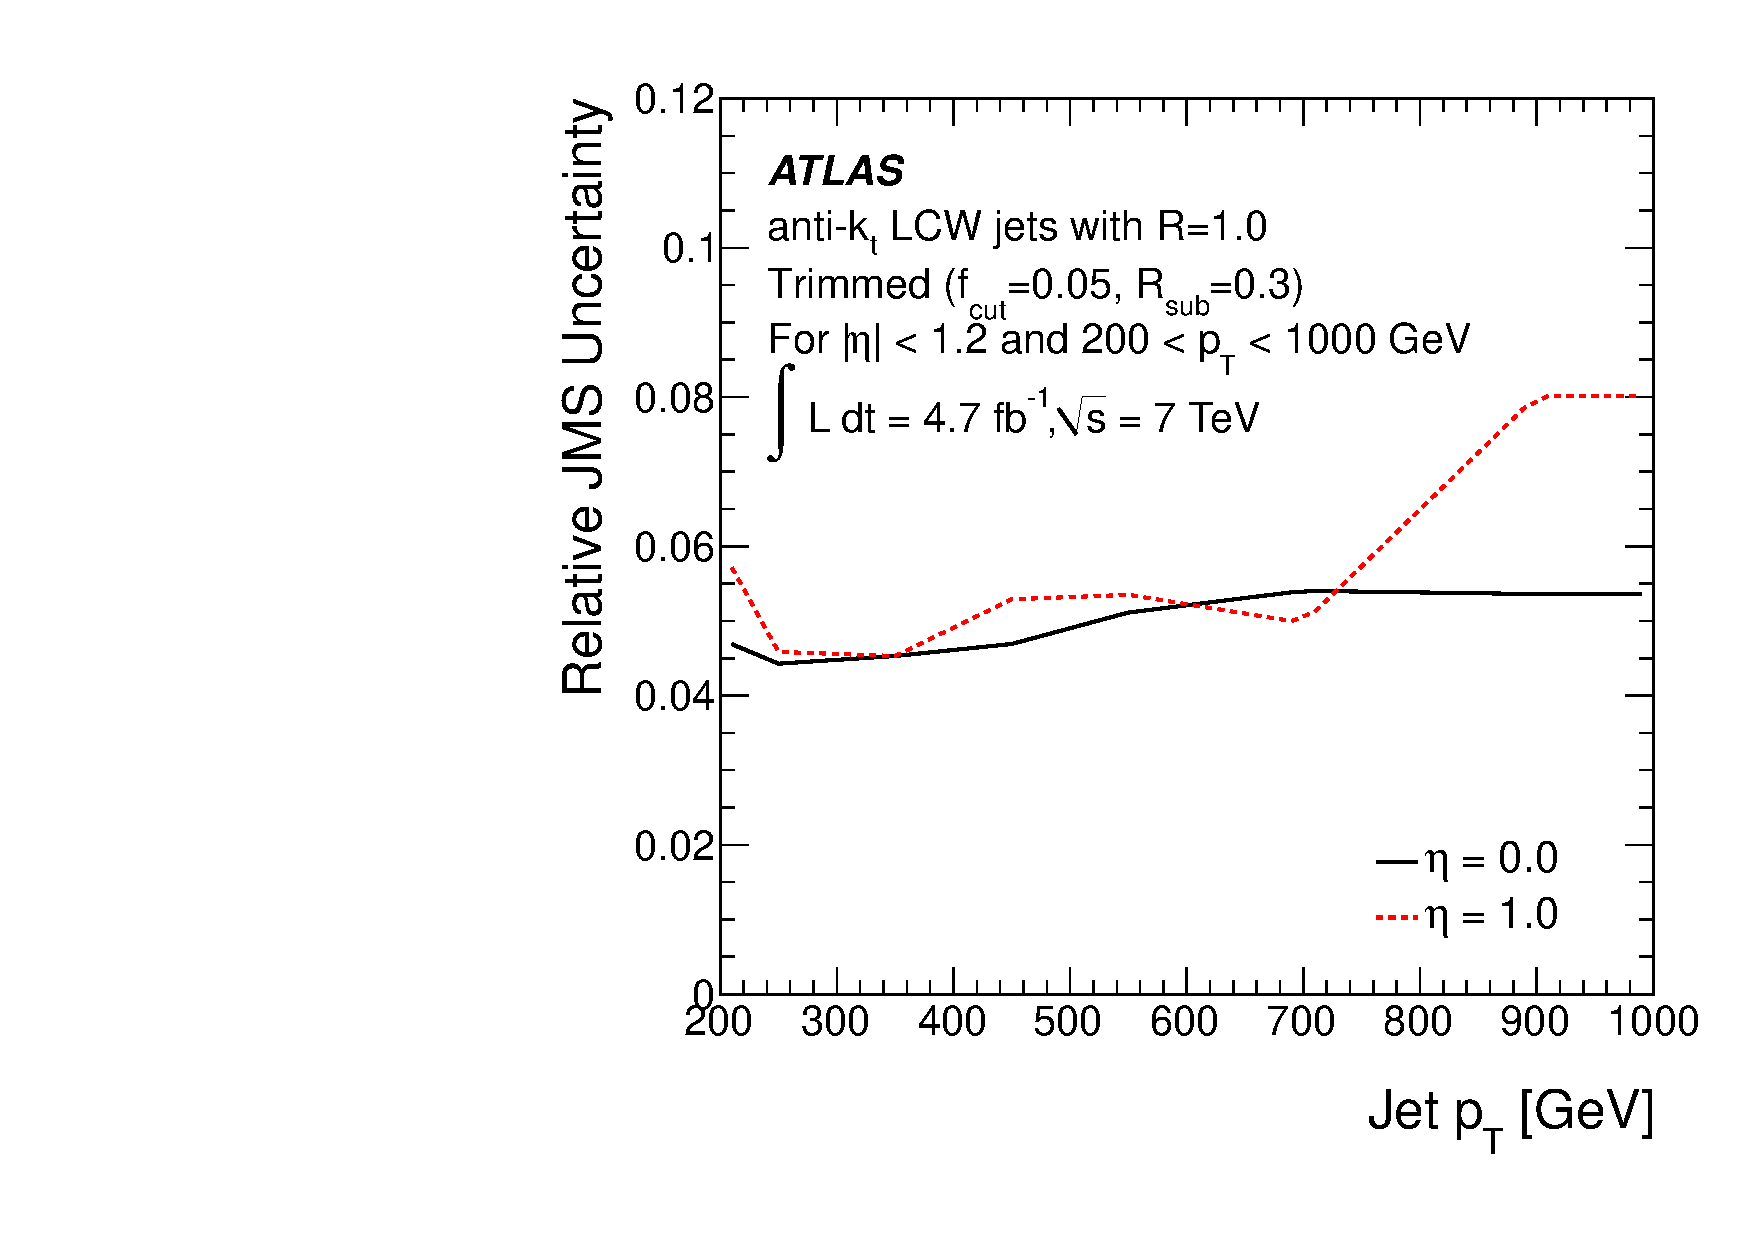
\includegraphics[width=0.45\textwidth]{fig_10b.pdf}}
\label{fig:jet-reconstruction:jms_uncertainty}
\caption{The jet track mass/ calo mass ratio in data and MC as a function of the jet mass, and the corresponding derived uncertainty as a function of jet \pt.}
\end{figure}


\section{Pileup Jet Tagging}
\label{jet-reconstruction:pileup-jet-tagging}

\section{Flavor Tagging}

\section{Quark/Gluon Discrimination}
	\subsection{Lots of subsections}
		...